%%%%%
%%%%%  Naudokite LUALATEX, ne LATEX.
%%%%%
%%%%
\documentclass[]{VUMIFTemplateClass}

\usepackage{indentfirst}
\usepackage{amsmath, amsthm, amssymb, amsfonts}
\usepackage{mathtools}
\usepackage{physics}
\usepackage{graphicx}
\usepackage{verbatim}
\usepackage[hidelinks]{hyperref}
\usepackage{color,algorithm,algorithmic}
\usepackage[nottoc]{tocbibind}
\usepackage{tocloft}

\usepackage{titlesec}

\usepackage{biblatex}
% \bibliography{Sem 8 Practice}
% \bibliography{internet}
%% norint pakeisti bibliografijos šaltinių numeravimą (skaitiniu arba raidiniu), pakeitimus atlikti VUMIFTemplateClass.cls 150 eilutėje

\usepackage{longtable}
\usepackage{booktabs}

% Custom for this work
\usepackage[acronym]{glossaries-extra}
\renewcommand{\acronymname}{Santrumpos}
\setabbreviationstyle{short-long}
\makenoidxglossaries

\glsaddkey
{ko}% key
{}% default value
{\glsentryko}% no link cs
{\Glsentryko}% no link ucfirst cs
{\glsko}% link cs
{\Glsko}% link ucfirst cs
{\GLSko}% link all caps cs

\glsaddkey
{kam}% key
{}% default value
{\glsentrykam}% no link cs
{\Glsentrykam}% no link ucfirst cs
{\glskam}% link cs
{\Glskam}% link ucfirst cs
{\GLSkam}% link all caps cs

\glsaddkey
{ka}% key
{}% default value
{\glsentryka}% no link cs
{\Glsentryka}% no link ucfirst cs
{\glska}% link cs
{\Glska}% link ucfirst cs
{\GLSka}% link all caps cs

\glsaddkey
{kuo}% key
{}% default value
{\glsentrykuo}% no link cs
{\Glsentrykuo}% no link ucfirst cs
{\glskuo}% link cs
{\Glskuo}% link ucfirst cs
{\GLSkuo}% link all caps cs

\glsaddkey
{kur}% key
{}% default value
{\glsentrykur}% no link cs
{\Glsentrykur}% no link ucfirst cs
{\glskur}% link cs
{\Glskur}% link ucfirst cs
{\GLSkur}% link all caps cs

\glsaddkey
{plko}% key
{}% default value
{\glsentryplko}% no link cs
{\Glsentryplko}% no link ucfirst cs
{\glsplko}% link cs
{\Glsplko}% link ucfirst cs
{\GLSplko}% link all caps cs

\glsaddkey
{plkam}% key
{}% default value
{\glsentryplkam}% no link cs
{\Glsentryplkam}% no link ucfirst cs
{\glsplkam}% link cs
{\Glsplkam}% link ucfirst cs
{\GLSplkam}% link all caps cs

\glsaddkey
{plka}% key
{}% default value
{\glsentryplka}% no link cs
{\Glsentryplka}% no link ucfirst cs
{\glsplka}% link cs
{\Glsplka}% link ucfirst cs
{\GLSplka}% link all caps cs

\glsaddkey
{plkuo}% key
{}% default value
{\glsentryplkuo}% no link cs
{\Glsentryplkuo}% no link ucfirst cs
{\glsplkuo}% link cs
{\Glsplkuo}% link ucfirst cs
{\GLSplkuo}% link all caps cs

\glsaddkey
{plkur}% key
{}% default value
{\glsentryplkur}% no link cs
{\Glsentryplkur}% no link ucfirst cs
{\glsplkur}% link cs
{\Glsplkur}% link ucfirst cs
{\GLSplkur}% link all caps cs

\setabbreviationstyle{long-short}

\bibliography{course_work}

\usepackage{mathtools}

\newcommand{\sectionbreak}{\clearpage}

\makeatletter
\renewcommand{\fnum@algorithm}{\thealgorithm}
\makeatother
\renewcommand\thealgorithm{\arabic{algorithm} algoritmas}


% --------------------------- Math Tools -------------------------------------

\DeclarePairedDelimiter\set\{\}

% Author's MACROS
\newcommand{\EE}{\mathbb{E}\,} % Mean
\newcommand{\ee}{{\mathrm e}}  % nice exponent
\newcommand{\RR}{\mathbb{R}}
\newcommand{\angl}[1]{\textit{(angl. #1)}}
\newcommand{\zr}[1]{(žr. \ref{#1}~pav.)}

\loadglsentries{structure/glossary.tex}

\begin{document}
\selectlanguage{lithuanian}

\onehalfspacing
\studijuprograma{Programų sistemų} %Studijų programą įrašyti kilmininko linksniu (pavyzdžiui – Programų sistemų, Finansų ir draudimų matematikos ir t. t.)
\darbotipas{Bakalauro baigiamasis darbas} % Bakalauro baigiamasis darbas arba magistro baigiamasis darbas
\darbopavadinimas{Varžymosi principais grįstų atakų aptikimas naudojant paaiškinamo dirbtinio intelekto metodą kenkėjiškų programų obfuskacijos kontekste}
\darbopavadinimasantras{Defense Against Adversarial Malware Obfuscation Attacks Using Explainable Artificial Intelligence}
\autorius{Liudas Kasperavičius}

%Autorių gali būti ir daugiau, tuo atveju, kiekvienas autorius rašomas iš naujos eilutės, ir pridedamas titulinis.tex arba dvigubasTitulinis.tex dokumentuose
%\antrasautorius{Vardas Pavardė} %Jei toks yra, kitu atveju ištrinti

\vadovas{prof. dr. Olga Kurasova}
\recenzentas{assoc. prof. Linas Petkevičius} %Jei toks yra žinomas, kitu atveju ištrinti
% \moksliniskonsultantas{pedagoginis/mokslinis vardas Vardas Pavardė} %Jei toks yra žinomas, kitu atveju ištrinti

\begin{titlepage}
\vskip 20pt
\begin{center}

\includegraphics[scale=0.55]{images/MIF.png}
\end{center}

\makeatletter

\vskip 20pt
\centerline{\bf \large \textbf{VILNIAUS UNIVERSITETAS}}
\vskip 10pt
\centerline{\large \textbf{MATEMATIKOS IR INFORMATIKOS FAKULTETAS}}
\vskip 10pt
\centerline{\large \textbf{\MakeUppercase{\@studijuprograma \space studijų programa}}}

\vskip 80pt
\centerline{\Large \@darbotipas}
\vskip 20pt
\begin{center}
    {\bf \LARGE \@darbopavadinimas}
\end{center}
\begin{center}
    {\bf \Large \@darbopavadinimasantras}
\end{center}
\vskip 80pt

\centering{\Large \@autorius}
\@ifundefined{@antrasautorius}{}
{
\vskip 10pt
\centering{\Large \@antrasautorius}
}
\vskip 20pt

\centering{
    \begin{tabular}{rcp{.7\textwidth}}
        {\Large Darbo vadovas} & {\Large :} & {\Large \@vadovas}\\[10pt]
        \@ifundefined{@moksliniskonsultantas}{}
            {
                {\Large Mokslinis konsultantas} & {\Large :} & {\Large \@moksliniskonsultantas}\\[10pt]
            }
        \@ifundefined{@recenzentas}{}
            {
                {\Large Recenzentas} & {\Large :} & {\Large \@recenzentas}\\[10pt]
            }
    \end{tabular}}


\vskip 110pt

\centerline{\large \textbf{Vilnius}}
\centerline{\large \textbf{\the\year{}}}

\makeatother

\newpage
\end{titlepage}
%\newgeometry{top=2cm,bottom=2cm,right=2cm,left=3cm}
\setcounter{page}{2}

\section*{Santrauka}

Šiame darbe nagrinėjamos \glspl{adversarial} prieš kenkėjiškų programų detektorius bei tokių atakų aptikimo ir apsisaugojimo nuo jų strategijos. Siekiant patobulinti jau esamus aptikimo metodus bei pritaikyti juos bet kokiems požymių vektoriams, siūloma sujungti \gls{mca} dimensijų mažinimo metodą ir \LIME -- \gls{ml} modelių sprendimų paaiškinimo metodą, kurie atitinka mokslinėje literatūroje minimas perspektyviausias \glsplko{adversarial} aptikimo strategijas. Atliekamas siūlomo metodo tyrimas nustatant jo tikslumą bei lyginant su prieš tai minėtomis \glsplko{adversarial} aptikimo strategijomis. Tyrimui pasitelkiamas \textit{MalGAN} karkasas kaip tokių atakų generatorius, kadangi šio karkaso naudojami dvejetainiai požymių vektoriai turėtų kelti daugiausia sunkumų esamiems apsisaugojimo nuo \glsplko{adversarial} metodams. Nustatyta, jog pasiūlytas metodas geba tiek apsaugoti nuo, tiek aptikti \glsplka{adversarial} efektyviau nei esami metodai. 

\clearpage
\section*{Summary}

This work analyses \glsen{adversarial}{adversarial attacks} against malware detectors as well as strategies of detection and defense against such attacks. With the goal to improve already existing detection methods and adapt them for use with any feature vectors, this work explores combining \gls{mca} dimensionality reduction method and \LIME -- a method for explaining \gls{ml} models' decisions as these are implementations of the most perspective strategies of defense against adversarial attacks mentioned in scientific literature. A study is conducted to determine the accuracy of the suggested method by comparing it with the aforementioned strategies of defense against \glsen{adversarial}{adversarial attacks}. \textit{MalGAN} framework is used for this study as the generator of such attacks since the binary vectors used by it should cause the most difficulty for existing strategies of defense. Experimental results show that the suggested method is able to both defend against and detect \glsen{adversarial}{adversarial attacks} more effectively and consistently than currently used methods.

%Turinys
\begin{spacing}{0.93}
    \tableofcontents
\end{spacing}
\onehalfspacing

\printnoidxglossaries
\clearpage

\sectionnonum{Įvadas}

Pastaraisiais metais kenkėjiškas kodas ir programos kuriamos itin sparčiai (\sim450000 kenkėjiškų programų per dieną \href{https://www.av-test.org/en/statistics/malware/}{2024 m. AV-TEST}\footnote{https://www.av-test.org/en/statistics/malware} duomenimis). Kenkėjiško kodo aptikimo programos, kurios tradiciškai remiasi programų \glsplkuo{signature}, nespėja atnaujinti pėdsakų duomenų bazių pakankamai greitai. Dėl to \gls{di}, tiksliau mašininio mokymosi (\gls{ml}), naudojimas kenkėjiškų programų ar kenkėjiško kodo aptikimo srityje tapo itin populiarus \cite{demetrioAdversarialEXEmplesSurvey2021}. Tačiau \gls{ml} modeliai, nors ir geba aptikti kenkėjiškas programas iš naujų, dar nematytų, duomenų, yra pažeidžiami \glsplkam{adversarial} \cite{castroAIMEDEvolvingMalware2019,huGeneratingAdversarialMalware2017,rosenbergGenericBlackBoxEndEnd2018,zhongReinforcementLearningBased2022}. Šių atakų principas yra \gls{ml} modelio --~klasifikatoriaus~-- \glsko{decisionBoundary} radimas -- žinant šią ribą pakanka pakeisti kenkėjiškos programos veikimą taip, kad \gls{ml} modelis priimtų sprendimą klasifikuoti ją kaip nekenksmingą \cite{demetrioAdversarialEXEmplesSurvey2021}. Nustatyta, jog šią ribą galima rasti tiek žinant klasifikatoriaus parametrus, tiek jų nežinant ir net turint labai ribotą prieigą prie klasifikatoriaus rezultatų (pvz., klasifikacijos rezultatą be tikimybių -- tokios sąlygos vadinamos \enquote{juodos dėžės} atvejai) \cite{fangEvadingMalwareEngines2019}.

Vis tik \glspl{adversarial} nėra neįveikiamos. Nuolat kuriami nauji jų aptikimo metodai, tokie kaip \gls{adverasrialRetraining}, gradientų slėpimas ir kt. Kiekvienas metodas turi savų stiprybių ir silpnybių bei dažniausiai remiasi viena iš specifinio \gls{ml} modelio įgyvendinimo savybių, kitaip tariant, nėra vieno geriausio, tinkamiausio ar teoriškai teisingo \glsplko{adversarial} aptikimo metodo. 
Tiksliau, nėra pačių \gls{ae} konstravimo teorinio modelio, dėl šio proceso kompleksiškumo, tad jų aptikimo strategijos teorinis modelis taip pat nėra žinomas \cite{chakrabortySurveyAdversarialAttacks2021}. Šiame darbe siekiama generalizuoti \gls{ae} aptikimą apjungiant panašiame kenkėjiškų programų aptikimo kontekste naudojamą \LIME \cite{ribeiroWhyShouldTrust2016} metodą ir kitas mokslinėje literatūroje aprašytas technikas.

\vspace{10pt}
\textbf{Tikslas} -- pritaikyti \LIME metodą sėkmingų varžymosi principais grįstų atakų aptikimui prieš kenkėjiškų programų detektorius vertinant bet kokius požymius.

\vspace{10pt}
\textbf{Uždaviniai}:
\begin{enumerate}
    \item Apžvelgti kenkėjiško kodo obfuskacijos metodus bei apsisaugojimo nuo jų strategijas.
    \item Pritaikyti \glsplko{adversarial} aptikimą dvejetainius požymių vektorius naudojantiems modeliams taikant dimensijų mažinimo metodus.
    \item Sukurti klasifikavimo proceso praplėtimą į jį įtraukiant \glspl{adversarial} aptikimą ir paaiškinimą su \LIME.
    \item Ištirti praplėsto klasifikavimo proceso tikslumą \angl{accuracy}.
\end{enumerate}
\section{Literatūros apžvalga}\label{sec:literature}
\subsection{Naudojami kenkėjiškų programų požymiai}\label{sec:literature:features}
\Glspl{adversarial} taikosi į \gls{ml} modeliais paremtus kenkėjiškų programų detektorius. Šie detektoriai yra klasifikatoriai -- pateiktį (programą) klasifikuoja kaip kenkėjišką \angl{malicious} arba nekenkėjišką \angl{benign}. Kadangi programos nėra fiksuoto dydžio, klasifikatoriai remiasi programų požymiais, kurie gaunami atliekant požymių ištraukimą \angl{feature extraction}. Laikoma, jog \enquote{juodos dėžės} atvejais sužinoti, kokius tiksliai požymius vertina kenkėjiškų programų detektorius, yra neįmanoma, tad \glsplko{framework} apibrėžimuose, priklausomai nuo jų specifikos ir tikslų, neretai pateikiami jų vertinami programų požymiai. Šiame poskyryje išskiriami ir klasifikuojami mokslinėje literatūroje minimi požymiai.

\subsubsection{\gls{pe} formato programų požymiai}\label{sec:literature:features:pe}
Išskiriami šie pagrindiniai \gls{pe} formato programų požymiai:
\begin{itemize}
    \item \textbf{\gls{dll} vardai (arba \gls{api} vardai \cite{huGeneratingAdversarialMalware2017})} \cite{zhongMalFoxCamouflagedAdversarial2024}. \gls{pe} faile turi būti nurodyti visi naudojami \gls{dll} ir jų \gls{api}. Prieš pradedant mokyti \gls{ml} modelį, atliekama visų turimų programų analizė ir nustatoma visų naudojamų \gls{dll} ar jų \gls{api} aibė $D$. Tarkime $|D| = n$. Tuomet, požymių vektorius programai, naudojančiai $X \subseteq D$ \gls{dll}, bus $n$-matis dvejetainis vektorius, kurio $i$-asis elementas yra $\begin{cases}
        0, \text{ jei } D_i \not \in X, \\
        1, \text{ jei } D_i \in X
    \end{cases}$ čia $D_i$ -- $i$-asis $D$ elementas.
    \item \textbf{\gls{pe} metaduomenys} \cite{andersonLearningEvadeStatic2018}. Tai visi \gls{pe} formato faile esantys metaduomenys, tokie, kaip sekcijų pavadinimai, sekcijų dydžiai, \textit{ImportTable} ir \textit{ExportTable} metaduomenys ir kt. Formuojant požymių vektorių skaičiuojama metaduomenų \gls{hashfunction}.
\end{itemize}

\subsubsection{Baitų lygio požymiai}\label{sec:literature:features:byte}
Baitų lygio požymiai gali būti ištraukiami iš bet kokio formato failų. Mokslinėje literatūroje minimi šie pagrindiniai baitų lygio požymiai:
\begin{itemize}
    \item \textbf{Prasmingų žodžių (angl. Strings) kiekis} \cite{andersonLearningEvadeStatic2018}. Prasmingus žodžius suprantame kaip turinčius prasmę žmogui \textit{(angl. human readable)}. Tai gali būti URL, failų keliai \textit{(angl. file paths)} ar registro raktų pavadinimai. Kadangi prasmingų žodžių kiekis tėra vienas skaičius, požymių vektorius dažniausiai formuojamas prijungiant ir kitus požymius.
    \item \textbf{Baitų/entropijos histograma} \cite{saxeDeepNeuralNetwork2015}. Specifinis metodas, užkoduojantis dažniausiai pasikartojančias baitų ir entropijos poras $n$ dimensijų vektoriumi.
    \item \textbf{$n$-gramos} \cite{zhuNgramMalGANEvading2022}. Dažniausiai sutinkamos skaitmeniniame natūraliosios kalbos apdorojime (\gls{nlp}). Tai yra $n$ žodžių junginiai, arba, sukompiliuotų programų apdorojimo kontekste, $n$ baitų junginiai. Nustatant požymių vektorių, visos $n$-gramos surikiuojamos pagal pasikartojimą programoje mažėjimo tvarka (\enquote{populiariausios} viršuje). Iš pirmų $m$ reikšmių sudaromas $m$-matis vektorius -- tai ir yra požymių vektorius.
\end{itemize}
\subsection{Perturbacijos}\label{sec:literature:perturbations}

Perturbacijos -- tai pagrindinis obfuskacijos metodas \gls{ae} kūrimui.
Perturbacijų tikslas yra pakeisti kenkėjiškos programos veikimą išsaugant
originalų funkcionalumą. Perturbacijos gali būti sudėtingos ir apimti visą
programą (pvz., visos programos užšifravimas ir pridėjimas prie kitos
programos), semantinės (pvz., tam tikrų mašininio kodo instrukcijų keitimas į
ekvivalentų rezultatą pasiekiančias) arba baitų lygio (pvz., nulinių baitų
pridėjimas programos gale) \cite{huGeneratingAdversarialMalware2017}. Perturbacijų parinkimas įeina į
\glsko{framework} apibrėžimą. Šiame poskyryje aptariamos mokslinėje
literatūroje minimos perturbacijos.
\subsubsection{Baitų lygio perturbacijos}\label{sec:literature:perturbations:byte}
Pačias paprasčiausias baitų lygio perturbacijas galima taikyti bet kokio formato failams, tačiau labiau prasmingos perturbacijos taikomos \gls{pe} formato failams. Išskiriamos šios pagrindinės baitų lygio perturbacijos:
\begin{itemize}
    \item \textbf{\textit{ARBE} (\textit{Append Random Bytes at the End})} \cite{fangEvadingMalwareEngines2019}. \gls{pe} formato failo gale pridedami atsitiktiniai baitai.
    \item \textbf{\textit{ARI} (\textit{Append Random Import})} \cite{fangEvadingMalwareEngines2019}. \gls{pe} formato failo \textit{ImportAddressTable} lentelėje pridedama atsitiktinai pavadinta biblioteka su atsitiktinai pavadinta funkcija.
    \item \textbf{\textit{ARS} (\textit{Append Randomly named Section})} \cite{fangEvadingMalwareEngines2019}. \gls{pe} formato failo \textit{SectionTable} lentelėje pridedamos atsitiktinės sekcijos (sekcijos ir jų tipai yra apibrėžti \gls{pe} formate).
    \item \textbf{\textit{RS} (\textit{Remove Signature})} \cite{fangEvadingMalwareEngines2019}. Sertifikato pašalinimas iš \gls{pe} formato failo \textit{CertificateTable} lentelės.
    \item \textbf{Naujas įeities taškas} \cite{andersonLearningEvadeStatic2018}. Prasidėjus programai, iškart peršokama nuo naujo įeities taško į originalųjį.
    \item \textbf{\textit{Header Fields}} \cite{demetrioAdversarialEXEmplesSurvey2021}. \gls{pe} formato failo \textit{PE Header} ir \textit{Optional Header} dalių specifinių laukų keitimas (pvz., sekcijos pavadinimo keitimas \cite{andersonLearningEvadeStatic2018}).
    \item \textbf{\textit{Partial DOS}} \cite{demetrioAdversarialEXEmplesSurvey2021}. \gls{pe} formato failo \textit{DOS Header} dalies pirmi 58 baitai po \textit{MZ} skaičiaus yra nenaudojami moderniose operacinėse sistemose, tad juos galima keisti.
    \item \textbf{\textit{Slack Space}} \cite{demetrioAdversarialEXEmplesSurvey2021}. Dėl \gls{pe} formato specifikos, kiekviena nauja sekcija turi prasidėti tam tikro skaičiaus, nurodyto \textit{PE Header} dalyje, kartotiniu nuo pradžios. Kompiliatoriai šį reikalavimą išpildo sekcijų gale pridėdami tiek nulinių baitų, kiek reikia teisingam sulygiavimui pasiekti. Būtent ši nulinių baitų erdvė gali būti keičiama be jokios įtakos originaliai programai.
    \item \textbf{\textit{Padding}} \cite{demetrioAdversarialEXEmplesSurvey2021}. Nulinių baitų pridėjimas failo gale.
    \item \textbf{\textit{Full DOS}} \cite{demetrioAdversarialEXEmplesSurvey2021}. Perturbacijos esmė tokia pat, kaip ir \textit{Partial DOS}, tik naudojami visi \textit{DOS} dalies baitai, išskyrus \textit{MZ} ir \textit{PE Offset} (\textit{Partial DOS} manipuliacijoms naudoja tik dalį tarp \textit{MZ} ir \textit{PE Offset}).
    \item \textbf{\textit{Extend}} \cite{demetrioAdversarialEXEmplesSurvey2021}. Pakeičiama \gls{pe} formato faile \textit{DOS} dalyje esanti \textit{PE Offset} reikšmė į didesnę\footnote{\label{footnote:structure}šios reikšmės padidinimas reiškia visos failo struktūros keitimą (\textit{DOS} dalis yra failo pradžioje). Būtina pakeisti visų sekcijų vietas nuo pradžios \angl{offset} jų metaduomenyse.}. Taip padidinama (išplečiama) visa \textit{DOS} dalis. Tolesnis perturbacijos principas yra toks pat, kaip ir \textit{Full DOS}.
    \item \textbf{\textit{Shift}} \cite{demetrioAdversarialEXEmplesSurvey2021}. \gls{pe} formato failuose kiekvienas sekcijos blokas prasideda su sekcijos vieta nuo pradžios \angl{offset}. Tarkime ši reikšmė yra $S$. Sekcijos kodas pradedamas vykdyti tik nuo adreso $P+S$, kur $P$ -- programos pradžios adresas. Vadinasi, padidinus\footnoteref{footnote:structure} $S$ per $n$, atsiranda $n$ baitų laisvos vietos iki sekcijos pradžios, kurią galima keisti be jokios įtakos programos veikimui.
\end{itemize}
\subsubsection{Semantinės perturbacijos}\label{sec:literature:perturbations:semantic}
Semantinių perturbacijų įgyvendinimas taip pat atliekamas baitų lygyje, tačiau šie pokyčiai turi aukštesnio lygio prasmę. Išskiriamos šios semantinės perturbacijos:
\begin{itemize}
    \item \textbf{Nereikalingų \hyperref[feature:dll]{DLL/API vardų} požymių pridėjimas} \cite{huGeneratingAdversarialMalware2017}. \gls{pe} formato faile \textit{ImportTable} lentelėje pridedami originalios programos nenaudojami \gls{dll}/\gls{api} vardai.
    \item \textbf{\textit{Binary Rewriting}} \cite{demetrioAdversarialEXEmplesSurvey2021}. Semantinis instrukcijų perrašymas. Pavyzdžiui, $A+B$ instrukcijos pakeitimas į $A-(-B)$.
\end{itemize}

\clearpage
\subsubsection{Kompleksinės perturbacijos}\label{sec:literature:perturbations:complex}
Kompleksinės perturbacijos yra pritaikomos tam tikriems tikslams. Obfuskacijos ir \glsplko{adversarial} tikslams literatūroje minimos šios kompleksinės perturbacijos:
\begin{itemize}
    \item \textbf{\textit{Obfusmal}} \cite{zhongMalFoxCamouflagedAdversarial2024}. Užšifruojama originalios programos kodo sekcija. Sukuriama ir originalios programos gale pridedama programa \textit{Shell.dll}, kurioje laikomas atšifravimo raktas, originalios programos kodo sekcijos adresas ir dydis. Be to, \textit{Shell.dll} geba atšifruoti originalios programos kodo sekciją ir jai perduoti kontrolę. \textit{Shell.dll} pridedama prie naudojamų \gls{dll}, o programos pradžios taškas nustatomas į \textit{Shell.dll} pradžios tašką. Iliustracija pateikiama \ref{fig:perturbations} pav.
    \item \textbf{\textit{Stealmal}} \cite{zhongMalFoxCamouflagedAdversarial2024}. Visa originali programa užšifruojama ir pridedama prie programos \textit{Shell.exe} galo. \textit{Shell.exe} geba atšifruoti originalią programą ir perduoti jai kontrolę. Iliustracija pateikiama \ref{fig:perturbations} pav.
    \item \textbf{\textit{Hollowmal}} \cite{zhongMalFoxCamouflagedAdversarial2024}. Užšifruojama visa originali programa. Ji pridedama prie kurios nors nekenksmingos programos galo. Prie šio junginio galo pridedama \textit{Hollow.dll} programa, kurios veikiamas panašus į \textit{Shell.exe} iš \textit{Stealmal}. Viso junginio pradžios taškas nustatomas į \textit{Hollowmal.dll} pradžios tašką. Iliustracija pateikiama \ref{fig:perturbations} pav.
\end{itemize}

\begin{figure}[h]
    \begin{small}
        \begin{center}
            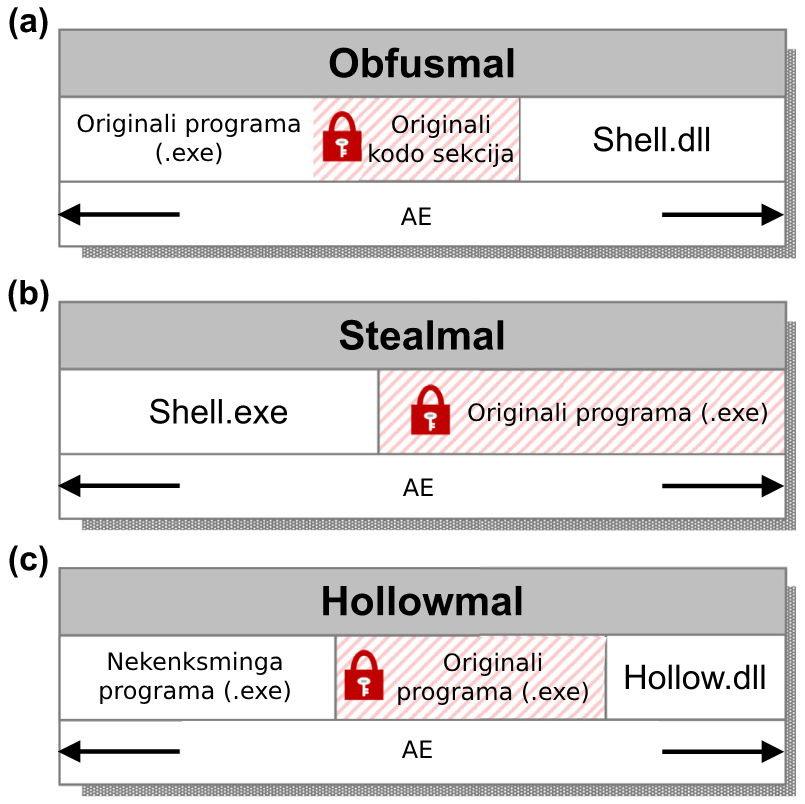
\includegraphics[width=0.4\textwidth]{images/complex-perturbations.png}
        \end{center}
        \caption{Obfusmal (a), Stealmal (b) ir Hollowmal (c) perturbacijų veikimo principų iliustracijos. Adaptuota iš \cite{zhongReinforcementLearningBased2022}}\label{fig:perturbations}
    \end{small}
\end{figure}
\clearpage
\subsection{GAN tipo modelių \glspl{framework}}\label{sec:literature:gan}

\gls{gan} modelių karkasai paremti generatyviniais priešiškais tinklais (\gls{gan}), kurių veikimo principas yra du neuroniniai tinklai (generatorius ir diskriminatorius), žaidžiantys \gls{zeroSumGame} \cite{chenInfoGANInterpretableRepresentation2016a}. Kenkėjiško kodo obfuskacijos kontekste ir ypač \enquote{juodos dėžės} atvejais, diskriminatorius atlieka \gls{surrogateModel} vaidmenį. Bendras \gls{gan} modelių mokymosi etapas yra tokia seka \cite{huGeneratingAdversarialMalware2017,zhuNgramMalGANEvading2022,zhongMalFoxCamouflagedAdversarial2024}:
\begin{enumerate}
    \item Generatorius, naudodamas požymių vektorių ir tokios pačios dimensijos
          \enquote{triukšmo} \angl{noise} vektorių, sugeneruoja perturbacijas.
    \item Originali kenkėjiška programa modifikuojama pagal perturbacijas (sukuriamas
          \gls{ae}).
    \item Diskriminatorius klasifikuoja sugeneruotą \gls{ae} (kenkėjiškas /
          nekenkėjiškas). Pagal klasifikacijos rezultatą skaičiuojamos diskriminatoriaus
          ir generatoriaus nuostolių funkcijos reikšmės (diskriminatoriaus nuostolių
          funkcijos reikšmė priklauso nuo tikro detektoriaus klasifikacijos).
    \item Visa seka kartojama nustatytą kiekį kartų.
\end{enumerate}

\begin{describeFramework}{MalGAN}{\cite{huGeneratingAdversarialMalware2017}}
    \introLastPar{
        Tai vienas iš pirmųjų ir populiariausių \gls{gan} tipo modelių \glsplko{framework}. \enquote{Juodos dėžės} detektoriai čia apibrėžiami kaip populiarūs \gls{ml} klasifikatoriai, tokie, kaip MLP \angl{Multilayer Perceptron}, RF \angl{Random Forest}, DT \angl{Decision Tree}, \gls{svm} \angl{Support Vector Machine}.
    }
    \purpose{
        Efektyviai išvengti \gls{ae} aptikimo, kai \gls{ml} kenkėjiškų programų detektoriaus įgyvendinimas nežinomas (\enquote{juodos dėžės} atvejis).
    }
    \surrogate{
        Daugiasluoksnis tiesioginio sklidimo neuroninis tinklas -- klasifikatorius. Įvestis -- programos požymių vektorius. Išvestis -- klasifikacija į kenksmingą arba nekenksmingą. Šis tinklas taip pat naudojamas kaip diskriminatorius \gls{gan} architektūroje.
    }
    \mainModel{
        Daugiasluoksnis tiesioginio sklidimo neuroninis tinklas. Įvestis -- programos požymių vektorius ir tokios pačios dimensijos \enquote{triukšmo} vektorius. Išvestis -- modifikuotas požymių vektorius. Šis tinklas naudojamas kaip generatorius \gls{gan} architektūroje.
    }
    \features{}{
        \textit{MalGan} straipsnyje \cite{huGeneratingAdversarialMalware2017} naudojami tik \gls{api} vardų požymiai, patenkantys į PE formato programų požymių kategoriją (žr. \ref{sec:literature:features:pe}), tačiau autoriai nurodo, jog gali būti naudojami bet kokie požymiai\footnote{\label{footnote:detector-assumptions}autoriai nagrinėja \enquote{juodos dėžės} atvejį su prielaida, jog detektoriaus naudojami požymiai yra žinomi.}.
    }
    \perturbations{}{
        Semantinės perturbacijos (\ref{sec:literature:perturbations:semantic}) --
        nereikalingų \gls{api} vardų požymių pridėjimas.
    }
\end{describeFramework}

\begin{describeFramework}{N-gram MalGAN}{\cite{zhuNgramMalGANEvading2022}}
    \introLastPar{
        Šis \gls{framework} remiasi \refFramework{MalGAN} karkasu ir siekia jį pagerinti.
    }
    \purpose{
        Supaprastinti, pagreitinti ir pagerinti \glsplka{adversarial}. Pašalinti prielaidas\footnoteref{footnote:detector-assumptions} apie detektorių \enquote{juodos dėžės} atvejais.
    }
    \surrogate{
        Surogatinio modelio veikimas ir architektūra tokia pati, kaip ir \refFramework{MalGAN}.
    }
    \mainModel{
        Pagrindinio modelio veikimas ir architektūra labai panašūs į \refFramework{MalGAN}, tačiau norėdami stabilizuoti mokymosi procesą, autoriai siūlo nenaudoti \enquote{triukšmo} vektoriaus. Vietoje to, generatoriaus išvestis ($n$-matis vektorius) modifikuojama nekeičiant pirmų $m$ dimensijų, o kitas $n-m$ pakeičiant nekenksmingų programų požymiais.
    }
    \features{}{
        Baitų lygio požymiai (\ref{sec:literature:features:byte}) -- $n$-gramos.
    }
    \perturbations{Autoriai neatliko eksperimentų su perturbuotomis programomis,
        tačiau pažymi, jog norint gauti sugeneruotus požymių vektorius užtenka pridėti
        reikiamus baitus programos gale. Tai atitinka
        \ref{sec:literature:perturbations:byte} apibrėžtą }{
        baitų lygio perturbaciją \textit{ARBE}, tik šiuo atveju pridedami baitai nebūtų
        atsitiktiniai, o norimos $n$-gramos.
    }
\end{describeFramework}

\begin{describeFramework}{MalFox}{\cite{zhongMalFoxCamouflagedAdversarial2024}}
    \introLastPar{
        \textit{\Name} taip pat remiasi \refFramework{MalGAN}, tačiau siekia kurti \gls{ae} realiomis sąlygomis, dėl to atlieka esminius pakeitimus.
    }
    \purpose{Generuoti \gls{ae}, kurių neaptiktų komerciniai detektoriai (prieš tai aptarti \glspl{framework} eksperimentams kaip nepriklausomą detektorių naudojo tokius \gls{ml} modelius, kaip \gls{svm}, \gls{knn}, \gls{gbdt} ir kt., bet ne komercinius detektorius). Šio \glsko{framework} detektorius yra \textit{VirusTotal} (viešai prieinama paslauga, agreguojanti virš 70 komercinių kenkėjiškų programų detektorių).}
    \surrogate{Surogatinis modelis, kaip ir kituose \gls{gan} tipo modelių karkasuose, naudojamas kaip diskriminatorius. Įvestis -- perturbuota programa. Išvestis -- klasifikacija į kenksmingą arba nekenksmingą. Įgyvendinimas -- konvoliucinis neuroninis tinklas (\gls{cnn}).}
    \mainModel{Standartinis \gls{gan} generatorius, požymių vektorių sujungiantis su \enquote{triukšmo} vektoriumi. Įgyvendinimas -- konvoliucinis neuroninis tinklas (\gls{cnn}).}
    \features{}{
        PE formato programų požymiai (\ref{sec:literature:features:pe}) -- \gls{dll}
        vardai. 
    }
    \perturbations{}{
        Visos kompleksinės perturbacijos (\ref{sec:literature:perturbations:complex}).
    }
\end{describeFramework}
\subsection{Skatinamojo mokymosi tipo modelių \glspl{framework}}\label{sec:literature:rl}

Skatinamojo mokymosi (\gls{rl}) modeliai susideda iš agento ir aplinkos.
Aplinka susideda iš informatyvių požymių ištraukimo metodo (\textit{angl.
    feature extraction}) ir kenkėjiškų programų detektoriaus. Šiuo atveju aplinkos
būsenų erdvė $S$ yra požymių vektorių erdvė. Agentas -- tai algoritmas ar
neuroninis tinklas, kurio tikslas yra surasti optimalią strategiją
\gls{policy}. Šiuo atveju strategijos veiksmų erdvė $A$ susideda iš
perturbacijų (žr. \ref{sec:literature:perturbations})
\cite{fangEvadingMalwareEngines2019}. Bendras \gls{rl} modelių mokymosi etapas
yra tokia seka \cite{fangEvadingMalwareEngines2019,
    zhongReinforcementLearningBased2022}:
\begin{enumerate}
    \item Agentas, naudodamas dabartinę aplinkos būseną ir praeito veiksmo atlygį
          \angl{reward}, parenka sekantį veiksmą iš galimų veiksmų aibės ir taiko
          mokymosi algoritmą (algoritmas priklauso nuo agento įgyvendinimo).
    \item Atliekamas veiksmas -- perturbuojama programa arba požymių vektorius (priklauso
          nuo \glsko{framework}).
    \item Gaunami aplinkos kitimo įverčiai -- nauja būsena ir atlygis, skaičiuojamas
          pagal detektoriaus klasifikacijos rezultatą.
    \item Seka kartojama tol, kol agentas nelaiko strategijos optimalia arba nustatytą
          kiekį kartų.
\end{enumerate}

\begin{describeFramework}{DQEAF}{\cite{fangEvadingMalwareEngines2019}}
    \introLastPar{
        Šis \gls{framework} taiko gilųjį skatinamąjį mokymąsi, kai agentas implementuojamas kaip gilusis neuroninis tinklas.
    }
    \purpose{Parodyti, jog \gls{ml} kenkėjiškų programų detektoriai, ypač modeliai, išmokyti prižiūrimu mokymusi, yra pažeidžiami \glsplkam{adversarial}.
    }
    \surrogate{\gls{rl} karkasuose nenaudojami surogatiniai modeliai. Kaip \enquote{juodos dėžės} detektorius pasirinktas \gls{gbdt} modelis.}
    \mainModel{Agentas implementuotas kaip gilusis $Q$-tinklas (\gls{cnn} praplėtimas, kai tinklas naudojamas kaip \glsko{qfunction} aproksimacija). Taip pat taikomas prioritetizuotas patirčių pakartojimo metodas \angl{prioritized experience replay}, kuomet agentas mokomas tik su aukštą atlygį gavusiais perėjimais ($S \times A$).}
    \features{Požymių vektorius taip pat apibrėžia visų būsenų erdvę $S$. Šiuo atveju $S = \mathbb{R}^{513}$.}{
        Baitų lygio požymiai (\ref{sec:literature:features:byte}) -- baitų/entropijos
        histograma. 
    }

    \perturbations{Perturbacijos apibrėžia visų galimų agento veiksmų
        erdvę $A$. Šiuo atveju $A = \set{0,1}^4$.}{
        Baitų lygio perturbacijos (\ref{sec:literature:perturbations:byte}):
        \begin{itemize}
            \item \textit{ARBE}
            \item \textit{ARI}
            \item \textit{ARS}
            \item \textit{RS}
        \end{itemize}
    }
\end{describeFramework}

\begin{describeFramework}{MalInfo}{\cite{zhongReinforcementLearningBased2022}}
    \introLastPar{
        \textit{\Name} remiasi \refFramework{MalFox}.
    }
    \purpose{Surasti optimalią obfuskacijos strategiją konkrečiai programai, pagal kurią sukurtas \gls{ae} nebūtų aptiktas komercinių kenkėjiškų programų detektorių.
    }
    \surrogate{\gls{rl} surogatinis modelis nenaudojamas. \enquote{Juodos dėžės} detektoriumi pasirinkti komerciniai detektoriai (\textit{VirusTotal}).
    }
    \mainModel{Agentas implementuotas kaip klasikiniai \gls{ml} algoritmai (konkrečiai dinaminis programavimas ir skirtumų laike \angl{temporal difference} algoritmas).
    }
    \features{Agentas nėra neuroninis tinklas ir požymių iš programos netraukia. Agentas mokosi tik iš perėjimų, o būsenų erdvė $S$ yra originali programa ir perturbuoti jos variantai. Teoriškai perturbuotų programos variantų galėtų būti be galo daug, tuomet $S = A^\infty, |S| = \aleph_0$, tačiau autoriai nurodo, jog daugiau nei 3 sluoksniai kompleksinių perturbacijų reikšmingai paveikia programos veikimo laiką, o tai gali \enquote{sukelti įtarimų} komerciniams detektoriams. Todėl pasirinkta $S = A^3$.
    }{}
    \perturbations{$A = \set{0,1,2,3}$}{
        \begin{itemize}
            \item \textit{Null} perturbacija -- naudinga tik formaliam pilnumui (atitinka nulinį $A$ veiksmą).
            \item Visos kompleksinės perturbacijos (\ref{sec:literature:perturbations:complex}),
                  t.~y. tokios pačios, kaip ir \refFramework{MalFox} \glsko{framework}. 
        \end{itemize}
    }
\end{describeFramework}
\subsection{Genetinių algoritmų tipo modelių \glspl{framework}}\label{sec:literature:genetic}

Genetinai algoritmai (\gls{genetic}) yra viena seniausių mašininio mokymosi
\gls{ml} apraiškų; jų veikimas paremtas evoliucija
\cite{castroAIMEDEvolvingMalware2019}. Kenkėjiškų programų obfuskacijai
\gls{ae} generavimas taikant \gls{genetic} yra tokia seka
\cite{yusteOptimizationCodeCaves2022}:
\begin{enumerate}
    \item Sukuriama pradinė populiacija (perturbacijos metodai pradinei populiacijai
          priklauso nuo \glsko{framework}).
    \item Atliekamas tinkamumo \angl{fitness} vertinimas.\label{enum:genetic:fitness}
    \item Atliekama selekcija -- dažniausiai pasirenkami geriausiai įvertinti
          populiacijos \gls{ae}, tačiau galimos ir kitos selekcijos strategijos.
    \item Atliekamas selekcijos atrinktų \gls{ae} kryžminimas (po 2) taip sukuriant naują
          \gls{ae}, turintį po dalį genų iš abiejų kryžmintų \gls{ae}.
    \item Tam tikrai daliai \gls{ae} atliekama dalies genų mutacija.
    \item Vertinama, ar sugeneruoti \gls{ae} atitinka kriterijus (vertina detektorius).
    \item Jei kriterijai nėra tenkinami, seka kartojama nuo \ref{enum:genetic:fitness}-o
          žingsnio.
\end{enumerate}

\begin{describeFramework}{AIMED}{\cite{castroAIMEDEvolvingMalware2019}}
    \purpose{\gls{ae} generavimo greičio padidinimas ir modelių kompleksiškumo sumažinimas, lyginant su \gls{gan} ir \gls{rl} tipo modelių karkasais.}
    \surrogate{Surogatinis modelis nenaudojamas. Naudojami \enquote{juodos dėžės} detektoriai yra \textbf{3 komerciniai} (\textit{Kaspersky, ESET, Sophos}) ir vienas \gls{ml} modelis -- \gls{gbdt}.}
    \mainModel{Klasikinis \gls{genetic} modelis -- veikimas visiškai atitinką bendrą seką. Tinkamumo \angl{fitness} vertinamas remiasi \gls{ae} požymių vektoriaus panašumu į originalios programos požymių vektorių (kuo mažiau panašūs, tuo tinkamumo įvertinimas didesnis).}
    \features{}{
        Baitų lygio požymiai \skyrius{sec:literature:features:byte} -- atskiras $n$-gramų
        atvejis, kai $n=1$.
    }
    \perturbations{}{ Baitų lygio
        perturbacijos\footnote{autoriai rėmėsi perturbacijomis, aprašytomis
            \cite{andersonLearningEvadeStatic2018}}
        \skyrius{sec:literature:perturbations:byte}. 
    }
\end{describeFramework}

\clearpage
\begin{describeFramework}{GAMMA}{\cite{demetrioFunctionalityPreservingBlackBoxOptimization2021}}
    \purpose{Efektyvus (neaptikimo šansų didinimas naudojant perturbacijas, paremtas nekenksmingomis programomis) \glsplko{adversarial} kūrimas.}
    \surrogate{Surogatinis modelis nenaudojamas. \gls{gbdt} ir \textit{MalConv} pasirinkti kaip \enquote{juodos dėžės} detektoriai.}
    \mainModel{Pagrindinė modelio idėja yra požymių ištraukimas iš nekenksmingų programų ir jų pridėjimas, naudojant tam pritaikytas perturbacijas, į kenksmingas programas kiekvienos populiacijos generavimo metu. Tinkamumo \angl{fitness} ir kriterijų vertinimas atliekamas naudojant detektorių ir pridėtų požymių dydį baitais (norima pridėti kuo mažiau požymių).}
    \features{}{
        \begin{itemize}
            \item \gls{pe} formato programų požymiai \skyrius{sec:literature:features:pe}.
            \item Kodas sekcijose (nestandartinis požymis).
        \end{itemize}
    }
    \perturbations{}{
        \begin{itemize}
            \item Visos baitų lygio perturbacijos \skyrius{sec:literature:perturbations:byte},
                  gebančios pridėti baitus.
            \item Autoriai pažymi, jog gali būti naudojama ir \gls{dll} / \gls{api} vardų
                  pridėjimo semantinė perturbacija \skyrius{sec:literature:perturbations:semantic}.
        \end{itemize}
    }
\end{describeFramework}
\subsection{Nevalidaus PE formato problema}\label{sec:literature:pe_invalid}

Andersonas ir kt.~\cite{andersonLearningEvadeStatic2018}, atlikdami eksperimentus su funkcionalumą išlaikančiomis perturbacijomis \gls{pe} formato failams, pastebėjo, jog ne visais atvejais perturbuotos programos veikia teisingai. Dėl \textit{Windows} operacinės sistemos \gls{pe} formato failų interpretavimo ir paleidimo specifikos, programas įmanoma parašyti tokiu būdu, jog pakeitus kodo ar kitų sekcijų turinį nekeičiant originalių mašininio kodo instrukcijų, programa neveiktų. Techniškai, programų rašymas tokiu būdu pažeidžia patį \gls{pe} formato standartą, tačiau šią praktiką neretai naudoja kenkėjiškų programų autoriai.

Norint visiškai išvengti nevalidaus \gls{pe} formato problemos tenka taikyti perturbacijas, nekeičiančias originalių programų, o taikančias kitokius obfuskacijos metodus. Iš \ref{sec:literature:perturbations} poskyryje aptartų perturbacijų, tokias sąlygas atitinka tik 2 kompleksinės perturbacijos (\ref{sec:literature:perturbations:complex}) -- \textit{Stealmal} ir \textit{Hollowmal}.
\subsection{\gls*{ae} perkeliamumas}\label{sec:literature:transfer}
Perkeliamumas \gls{di} modeliuose dažniausiai suprantamas kaip žinių perkeliamumas \angl{knowledge transferability}. Tačiau tiriant \glsplka{adversarial} buvo pastebėtas ir \gls{ae} perkeliamumas \angl{adversarial sample transferability}. Tai reiškia, jog gebant sukurti \gls{ae}, kuriuos neteisingai klasifikuoja vienas modelis, tikėtina, jog kitas (tos pačios paskirties) modelis taip pat klasifikuos \gls{ae} neteisingai. Be to, nustatyta, jog \gls{ae} perkeliamumo savybė galioja skirtingų architektūrų modeliams \cite{demetrioAdversarialEXEmplesSurvey2021}. Šia savybe remiasi visos \enquote{juodos dėžės} atvejams pritaikytos atakos.
\section{\gls{mca} ir \LIME \gls{ae} aptikimo metodų sintezė}\label{sec:method}

Autoriaus siūlomas \gls{ae} aptikimo metodas yra apjungti \gls{mca} dimensijų mažinimo metodą bei \LIME pritaikymą \gls{ae} aptikimui su tam tikromis modifikacijomis (\ref{sec:method:mods}). Kadangi \gls{mca} ir \LIME atitinka bazės keitimo \skyrius{sec:literature:defense:basis}{} ir perkeliamumo blokavimo \skyrius{sec:literature:defense:blocking}{} \gls{ae} aptikimo strategijas, kurios iš aptartų yra perspektyviausios -- jų sinteze tikimasi gauti dar tikslesnį \gls{ae} aptikimo metodą \zr{fig:original}.

\subsection{\LIME pritaikymo \gls{ae} aptikimui metodo modifikacijos}\label{sec:method:mods}
\ref{sec:literature:defense:ids} skyriuje siūlomas \LIME pritaikymas remiasi svarbiausių (didžiausią įtaką \gls{ml} modelio sprendimų priėmimui turinčių) požymių analize. Svarbiausi požymiai laikomi pirmieji 10 \cite{tcydenovaDetectionAdversarialAttacks2021}. Nors autoriai neaprašo kaip pasirenkama tokia konstanta, akivaizdu, jog ji nėra tinkama visiems atvejams. Pavyzdžiui, turint žymiai daugiau požymių, ši konstanta gali būti per maža. Tokia problema ypač aktuali kai analizuojami kategoriniai požymiai, turintys daug kategorijų (dažniausiai koduojami kaip dvejetainiai vektoriai -- \Angl{one-hot encoding}). Dėl šios priežasties, autoriaus siūlymas yra \enquote{svarbiais} laikyti visus požymius ir mokymo fazės pabaigoje apskaičiuoti šių požymių įtakos \gls{ml} modelio sprendimo priėmimui statistikas (vidurkį ir standartinį nuokrypį). Tuomet aptikimo fazėje naudoti $3 \sigma$ taisyklę \cite{pukelsheimThreeSigmaRule1994} \ty jei bent vieno požymio įtaka \gls{ml} sprendimo priėmimui nukrypsta per 3 standartinius nuokrypius nuo duotojo požymio vidurkio -- laikyti, jog analizuojama įvestis buvo obfuskuota.

\subsection{\LIME branduolio pločio pasirinkimas}

\LIME branduolio plotį \skyrius{sec:literature:lime}{} gali padėti nustatyti duomenų vizualizacijos ar kita duomenų analizė. Tai atlikti nėra sudėtinga, kai požymių vektoriaus dimensija nedidelė arba požymiai yra skaitiniai, tačiau turint kategorinius požymius ir atsižvelgiant į jų kodavimą dvejetainiais vektoriais, parinkti tinkamą \LIME branduolio plotį gali būti sudėtinga. Taikant \gls{mca} transformaciją neretai užtenka branduolio pločio vertę parinkti pagal pirmų dviejų komponenčių skalę, kadangi šios dvi komponentės apibūdina didžiausią inerciją \zr{fig:scree}.

\begin{figure}[h]
    \captionsetup{justification=centering}
    \begin{minipage}{0.48\textwidth}
        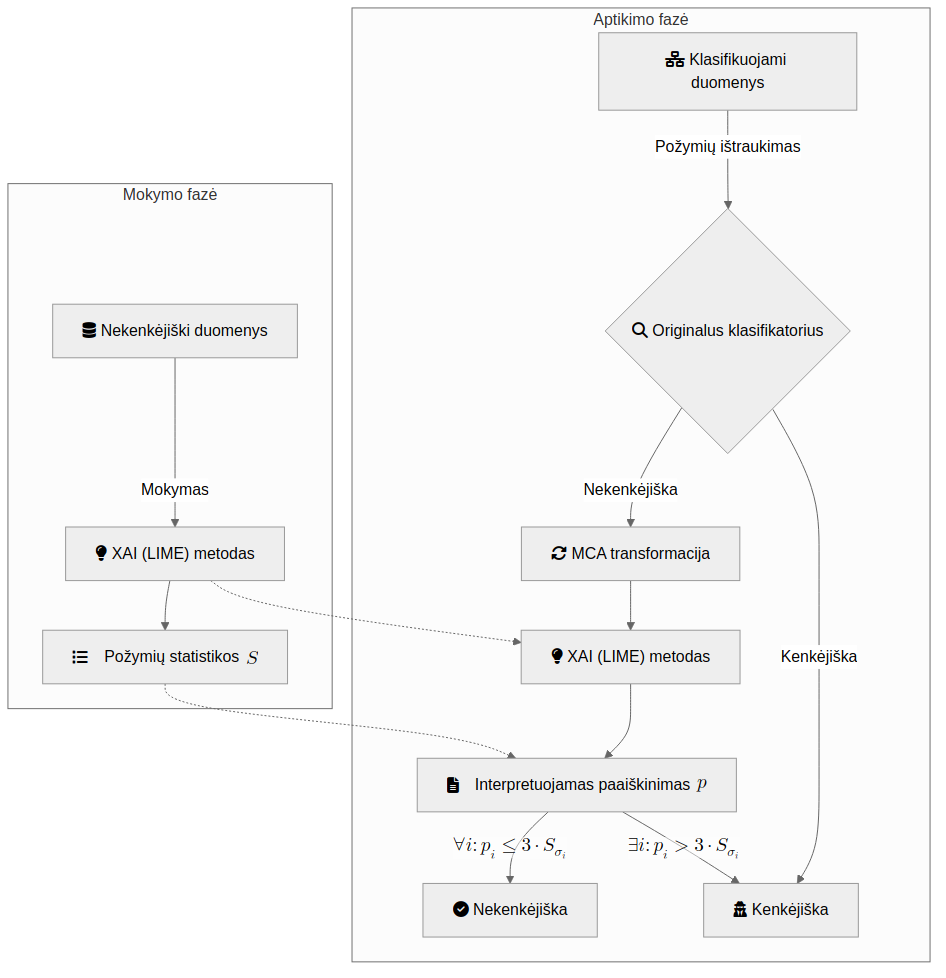
\includegraphics[width=0.95\textwidth]{images/original.png}
        \caption{\LIME ir \gls{mca} sintezės \gls{ae} aptikimo metodo iliustracija}
        \label{fig:original}
    \end{minipage}
    \begin{minipage}{0.48\textwidth}
        \centering
        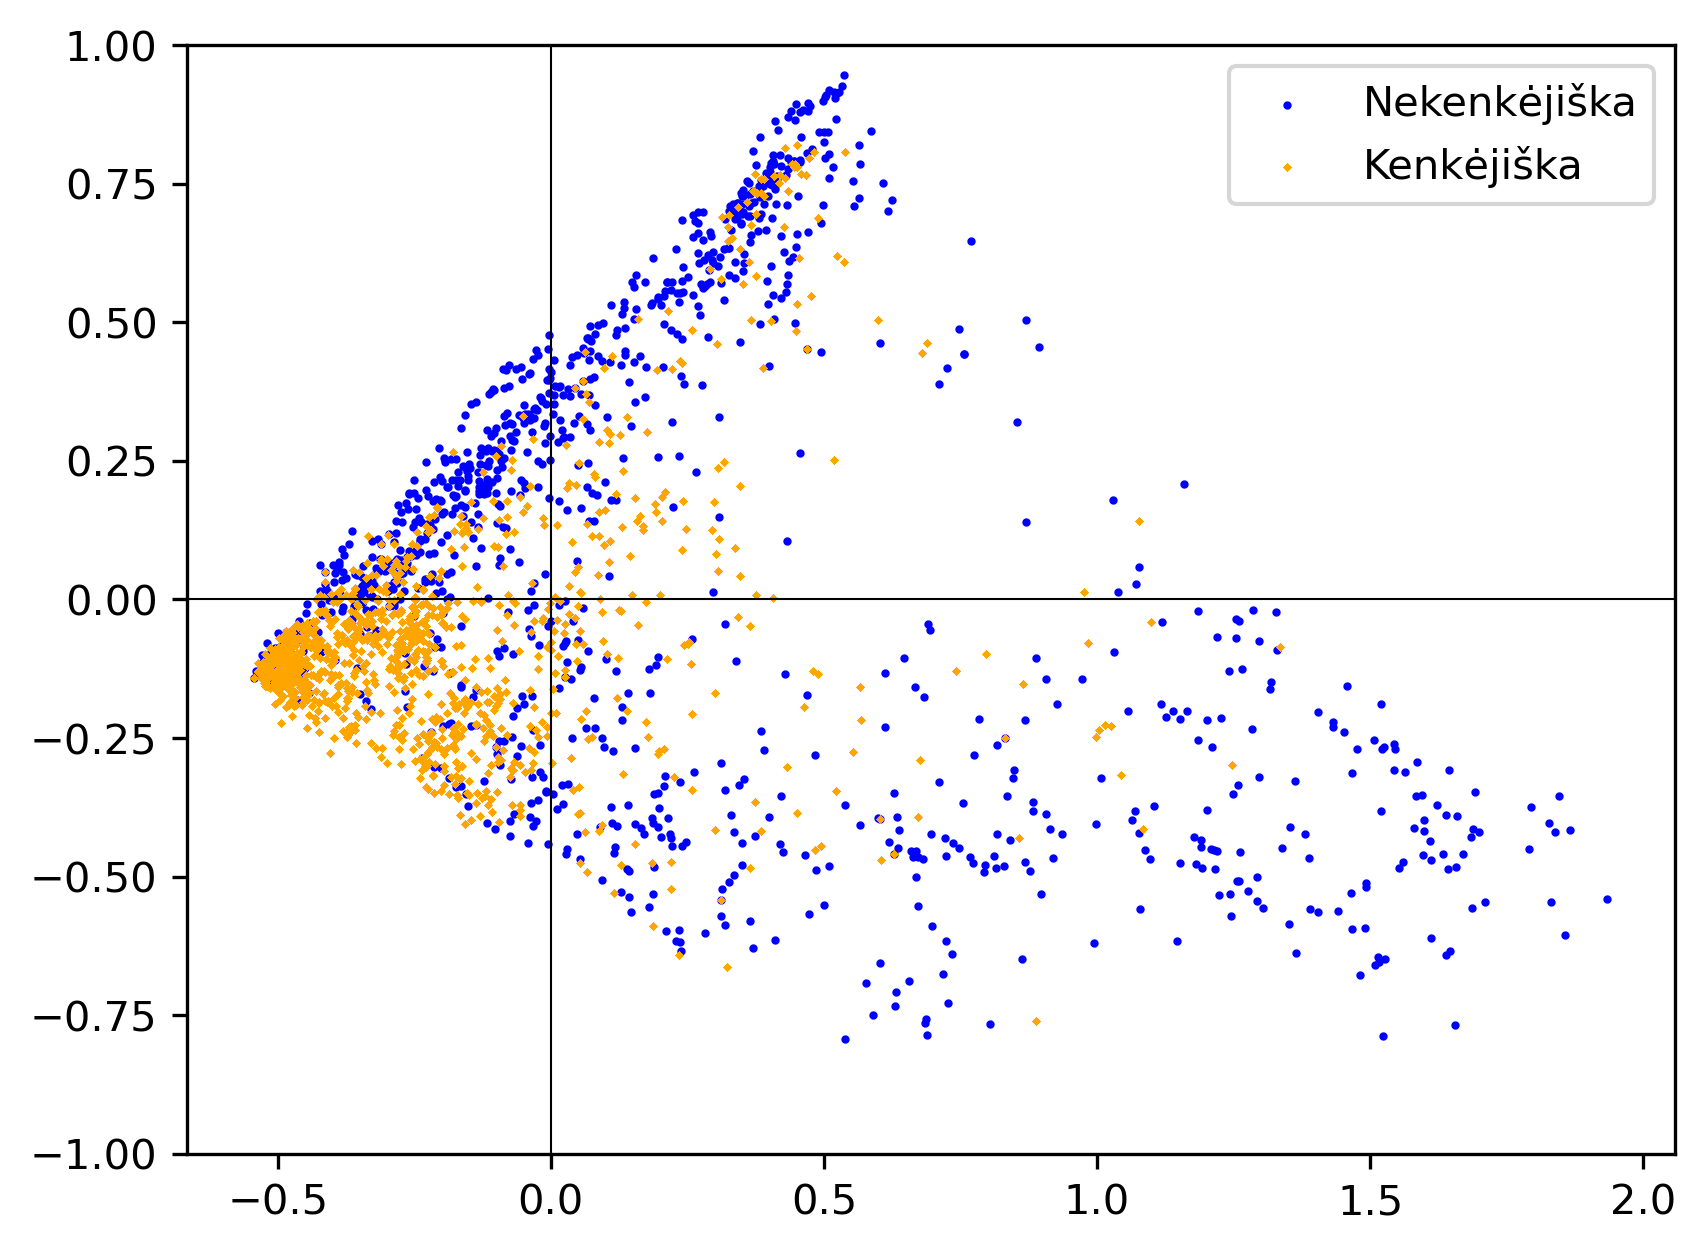
\includegraphics[width=\textwidth]{images/mca_scatter.png}
        \caption{Pirmųjų dviejų \gls{mca} transformacijos komponenčių pavyzdys}
        \label{fig:scree}
    \end{minipage}
\end{figure}


% Problem with selecting N components to explain
% Problem with binary feature vectors
% Synthesis of MCA and LIME (original)
% Method flow diagram (adaptation)
% Importance of keeping obfuscation detection hidden (original)
\section{Lyginamoji metodų analizė}\label{sec:experiments}

Lyginamosios analizės tikslas -- ištirti kenkėjiškų programų detektorių tikslumą \glsko{adversarial} sąlygomis. Lyginami originalus (nepakeistas) detektorius, autoriaus siūlomas \LIME ir \gls{mca} sintezės metodas (\ref{sec:method}) bei atskiros jo sudedamosios dalys: \LIME metodo pritaikymas \gls{ae} aptikimui (\ref{sec:literature:defense:ids}) ir \gls{mca} transformacijos klasifikatorius (\ref{sec:literature:mca}).

% Describe how the experiments are performed

\subsection{Tyrimo metodika}

Visa tyrimo metodika pavaizduota \ref{fig:methodology}-ame pav. Tyrimui pasirinktas \SLEIPNIR \cite{al-dujailiAdversarialDeepLearning2018} duomenų rinkinys, kuriame yra $34995$ kenkėjiškų programų ir $19696$ nekenkėjiškų programų pavyzdžių, užkoduotų $22761$-mačiais dvejetainiais vektoriais. Iš šio rinkinio pasirinkta po $1500$ unikalių kenkėjiškų ir nekenkėjiškų programų pavyzdžių paliekant pirmas $200$ komponenčių -- taip gaunamas subalansuotas duomenų rinkinys. Šis rinkinys toliau skeliamas į mokymo ir testavimo aibes santykiu $4:1$.
Eksperimentams atlikti paruošiamos šios priemonės:
\begin{enumerate}
    \item Testavimo duomenų aibė, iš kurios sudaromas trijų tipų programų požymių srautas: nekenkėjiškos, kenkėjiškos, kenkėjiškos-obfuskuotos.
    \item \textit{MalGAN} \cite{huGeneratingAdversarialMalware2017} \gls{ae} generatorius. Pasirinkimo motyvacija pateikiama \ref{sec:method:malgan} poskyryje.
    \item Kenkėjiškų programų detektorius (klasifikatorius).
    \item \Glsplko{adversarial} aptikimo komponentas
    \begin{itemize}
        \item Naudojantis originalius požymius.
        \item Naudojantis \gls{mca} transformuotus požymius \skyrius{sec:method}.
    \end{itemize}
\end{enumerate}

\noindent
Su šiais įrankiais atliekami 4 eksperimentai \textbf{aplinkoje su \glsplkuo{adversarial}}:
    \begin{enumerate}
        \item Bazinis atvejis -- originalaus klasifikatoriaus tikslumo nustatymas.
        \item Klasifikatoriaus, naudojančio \gls{mca} transformuotus požymius, tikslumo nustatymas.
        \item Klasifikatoriaus praplėtimo su modifikuoto \LIME metodo pritaikymu \glsplko{adversarial} aptikimui tikslumo nustatymas.
        \item Klasifikatoriaus praplėtimo su \LIME ir \gls{mca} metodų sinteze \glsplko{adversarial} aptikimui tikslumo nustatymas.
    \end{enumerate}

\begin{figure}[h]
    \centering
    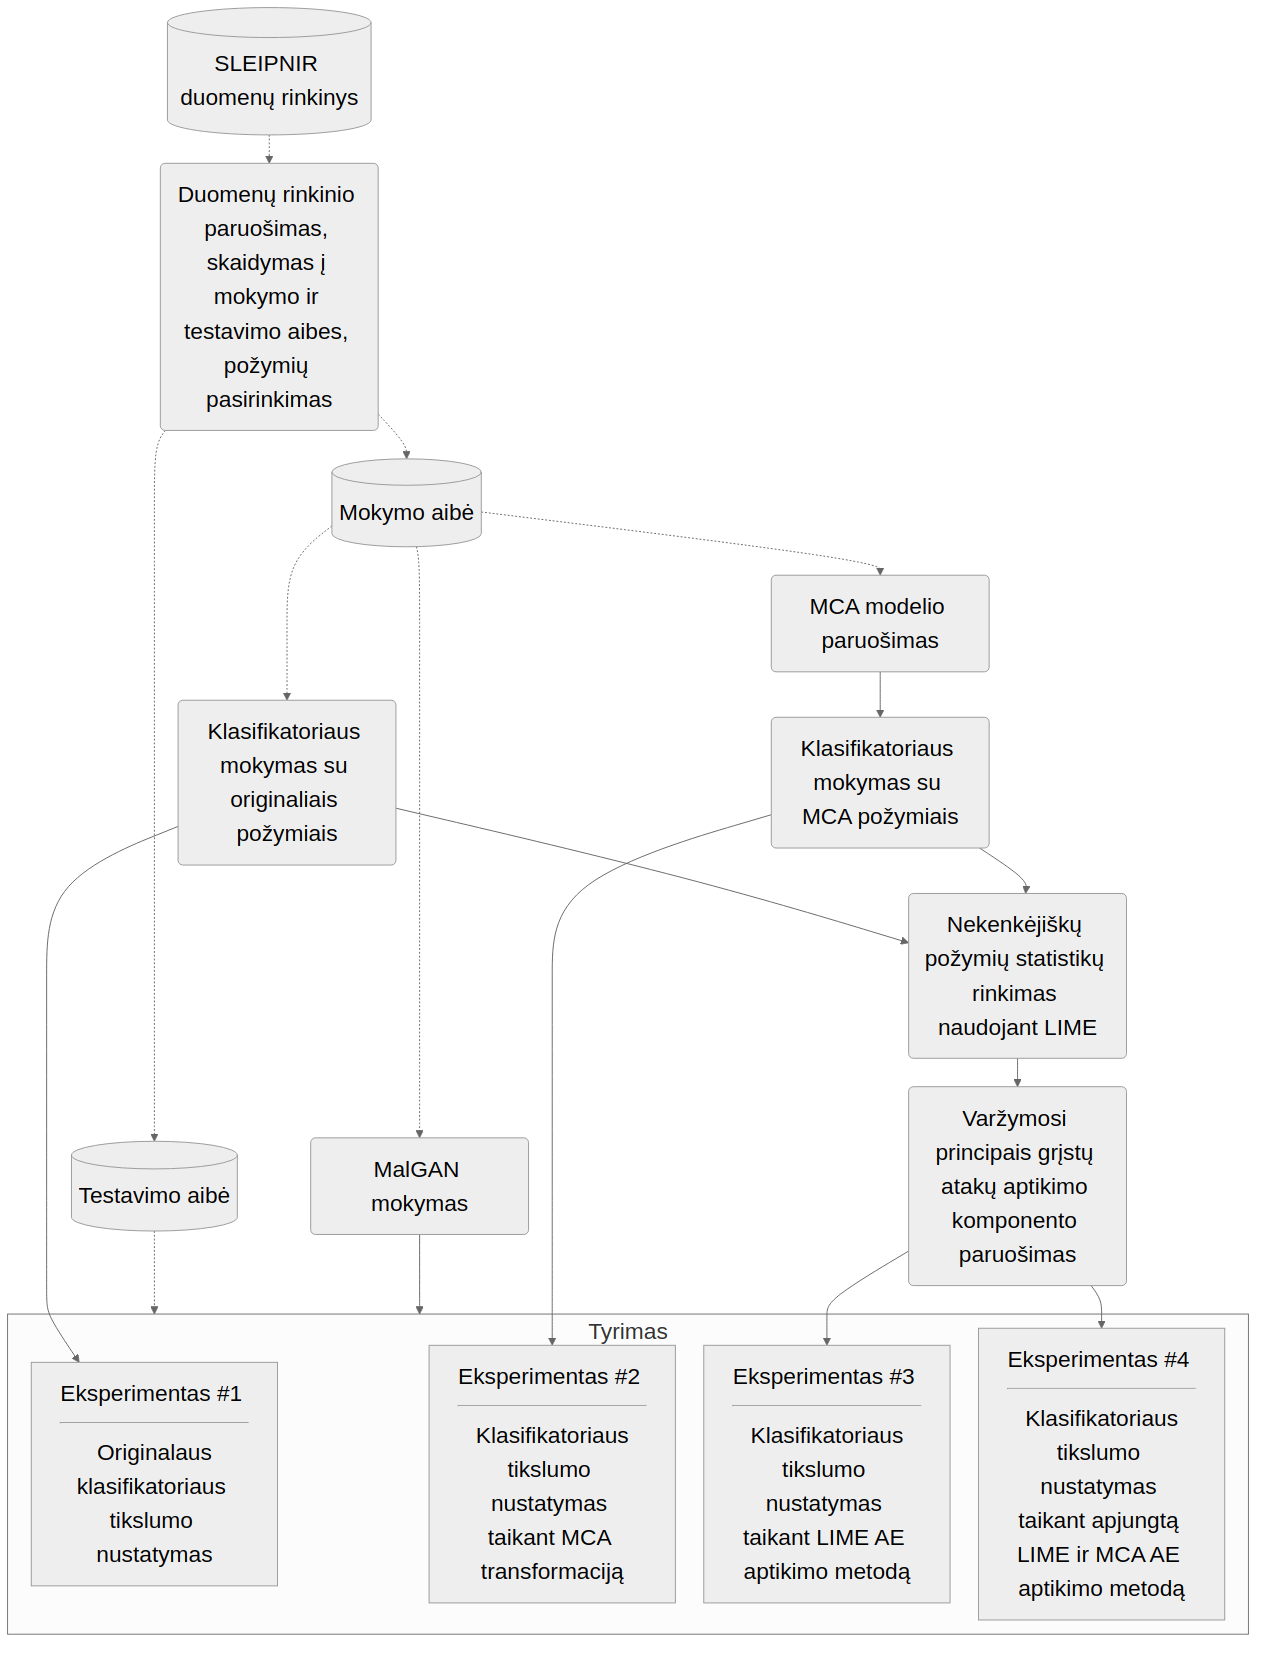
\includegraphics[width=\textwidth]{images/methodology.png}
    \caption{Tyrimo metodika}
    \label{fig:methodology}
\end{figure}

\subsection{\Glsplko{adversarial} \glsko{framework} pasirinkimas}\label{sec:method:malgan}

Tyrimui pasirinktas \refFramework{MalGAN} \gls{framework} dėl šių priežasčių:
\begin{itemize}
    \item \gls{gan} yra vieni iš perspektyviausių ir efektyviausių \gls{ml} modelių \gls{ae} generavimui.
    \item \textit{MalGAN} yra plačiai naudojamas kaip bazinis modelis tolimesniems tyrimas, yra kelios atviro kodo repozitorijos\footnote{Šiam tyrimui pasirinkta https://github.com/ZaydH/MalwareGAN repozitorija, kaip pradinis \textit{MalGAN} įgyvendinimas}, įgyvendinančios šį \glska{framework}.
    \item \textit{MalGAN} naudoja dvejetainius požymių vektorius. Būtent tokie požymiai turėtų kelti sunkumų esamiems \gls{ae} aptikimo metodams \skyrius{sec:method:mods}.
\end{itemize}

\clearpage
\subsection{\gls{mca} komponenčių pasirinkimas}\label{sec:method:mca_comp_selection}
Komponenčių pasirinkimas yra \ref{fig:methodology}-ame pav. minimo \gls{mca} modelio paruošimo dalis. Komponenčių pasirinkimui \ty jų kiekio pasirinkimui nėra apibrėžto \enquote{teisingo} metodo \cite{abdiPrincipalComponentAnalysis2010}. Dažniausiai siūlomi metodai yra tik didesnių už $1$ tikrinių reikšmių pasirinkimas ir \textit{alkūnės} \angl{scree / elbow} metodas. Šie metodai netiko, nes juos taikant paliktos \gls{mca} komponentės nepaaiškintų net pusės visos \glsko{inertia}: visos tikrinės reikšmės analizuojamuose mokymo duomenyse yra $<1$, o alkūnės taške sukaupta \gls{inertia} yra $\num{47,62} \%$ \zr{fig:inertia}. Taigi, pasirinkti 2 nestandartiniai \gls{mca} komponenčių kiekio kriterijai: 

\noindent
\begin{minipage}[l]{0.48\textwidth}
    \vspace{-2cm}
    \begin{itemize}[leftmargin=*]
        \item sukaupta \gls{inertia} $\ge 75\%$,
        \item išmokyto klasifikatoriaus tikslumas $\hat{a}$ nemažesnis nei originalaus klasifikatoriaus tikslumas $a$ $5\%$ intervale ($\hat{a} \ge a - 5\%$), kai įvesčių srautas normalus (nėra obfuskuotų programų požymių -- \gls{ae}). Šiuo atveju $\hat{a} \ge \num{\mathOp{\accNoAttackNormal - 0.05}}$ \Zr{tbl:safe:original:metrics}
    \end{itemize}
\end{minipage}
\hspace{0.02\textwidth}
\begin{minipage}{0.5\textwidth}
    \centering
    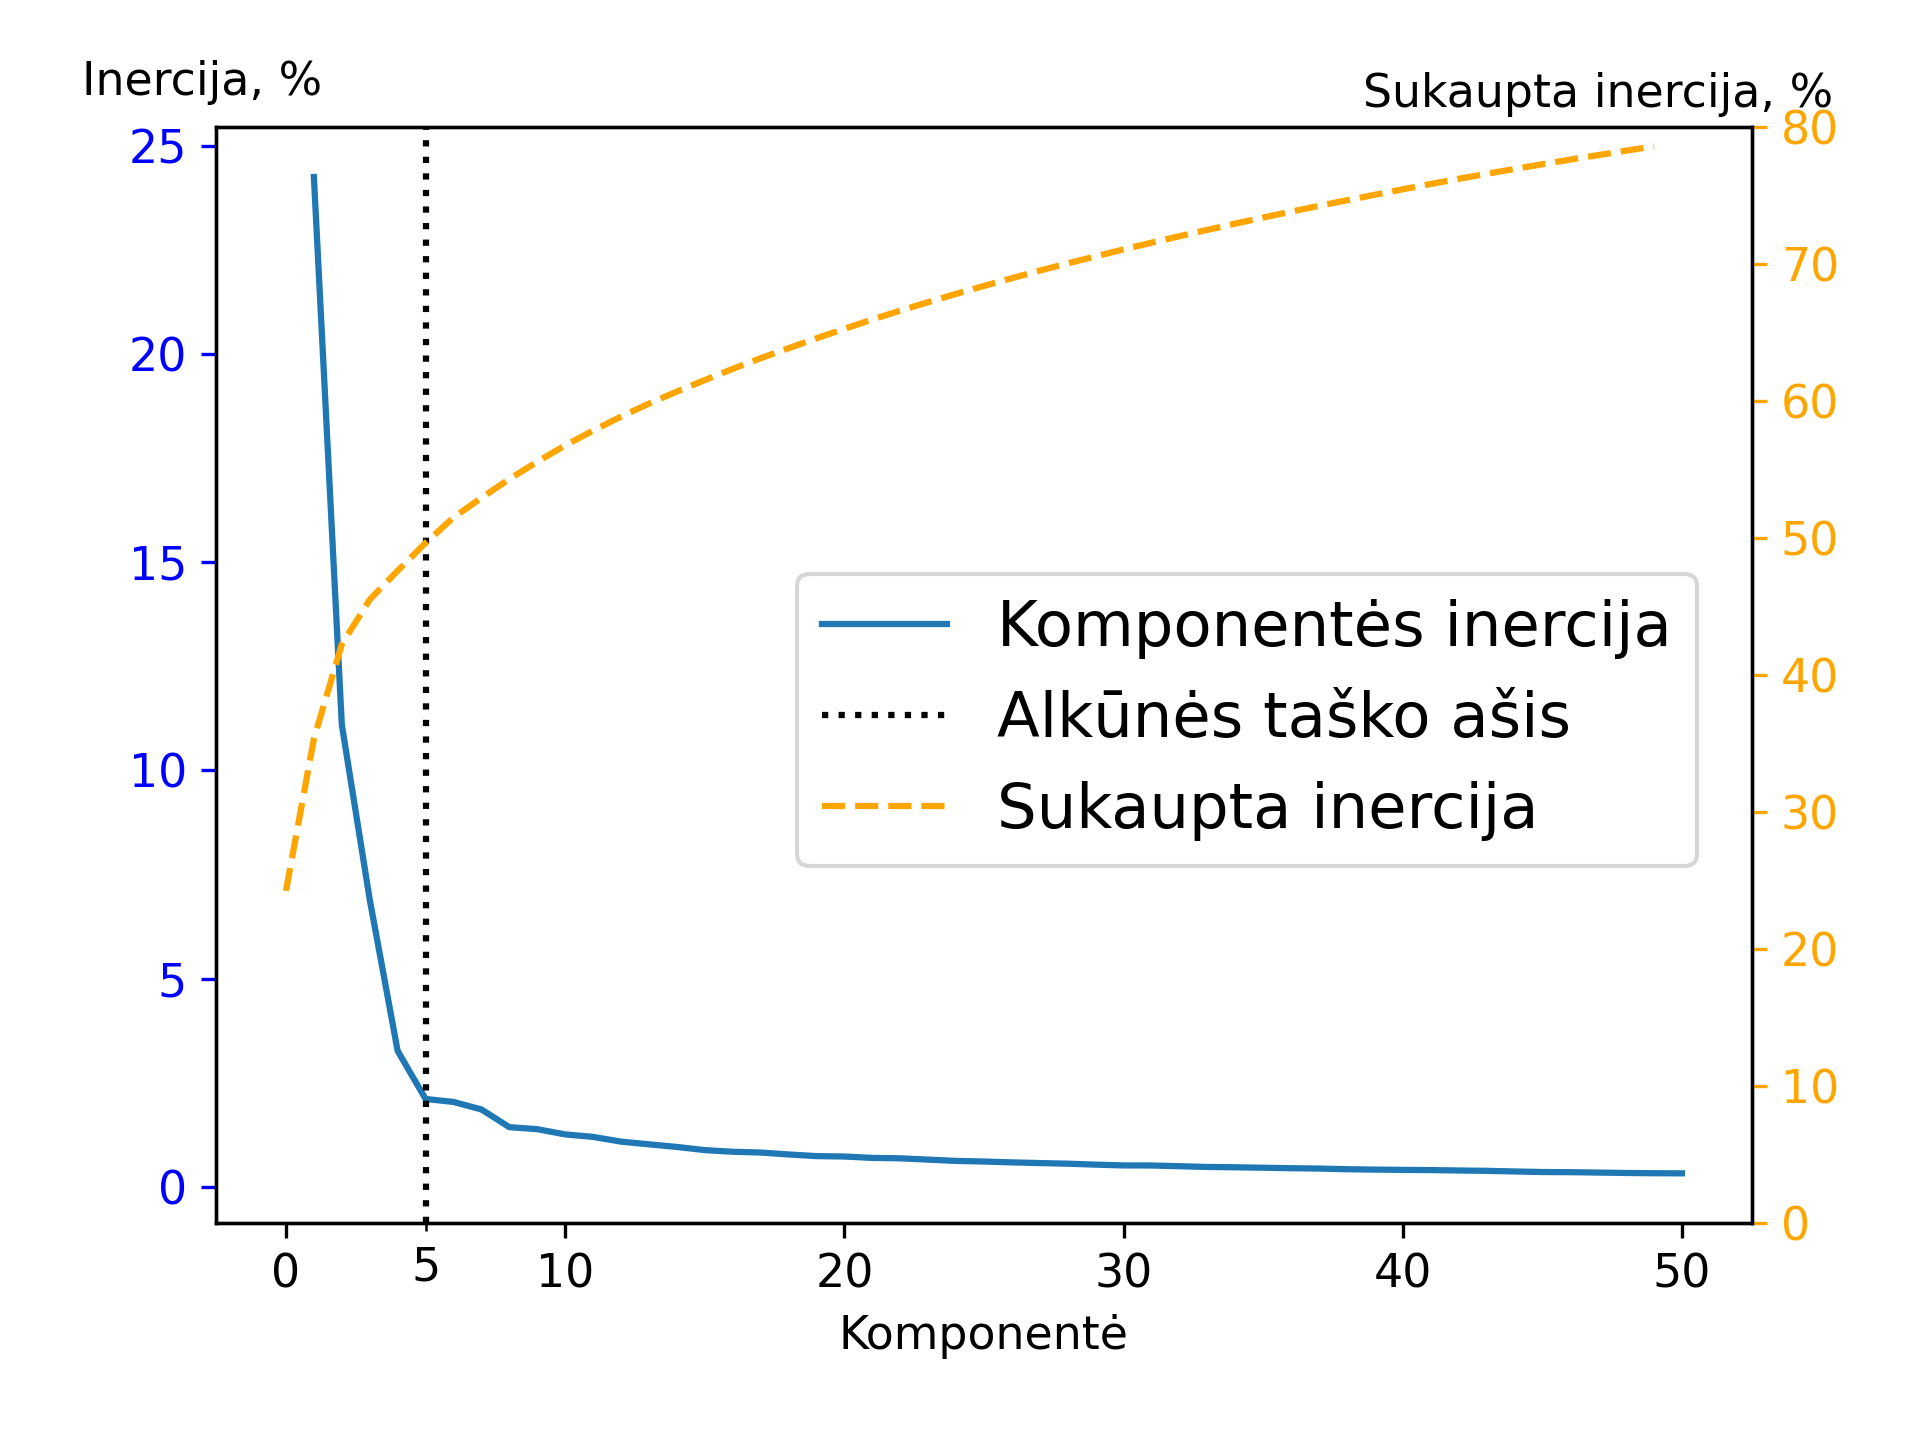
\includegraphics[width=\textwidth]{images/scree.png}
    \vspace{-1cm}
    \captionof{figure}{\textit{Alkūnės} analizė \gls{mca} inercijai}
    \label{fig:inertia}
\end{minipage}

\begin{table}[h]
    \centering
    \caption{Originalaus klasifikatoriaus metrikos, kai nevykdoma \gls{adversarial}}
    \exptable[\accNoAttackNormal]{tables/original_no_attack.csv}
    \label{tbl:safe:original:metrics}
\end{table}
\begin{table}[h]
    \centering
    \caption{\gls{mca} klasifikatoriaus metrikos, kai nevykdoma \gls{adversarial}}
    \exptable[\accNoAttackMca]{tables/mca_no_attack.csv}
    \label{tbl:safe:mca:metrics}
\end{table}

\def\accumulatedInertia{$78,57\%$}

\ref{tbl:safe:mca:metrics}-oje lentelėje pavaizduotos \gls{mca} transformacijos klasifikatoriaus metrikos gaunamos pasirinkus 50 komponenčių (suspaudimo santykis $4:1$), kurių sukaupta \gls{inertia} yra \accumulatedInertia. Kadangi \accumulatedInertia $\;> 75\%$ ir $\num{\accNoAttackMca} > \num{\mathOp{\accNoAttackNormal - 0.05}}$, abu \gls{mca} komponenčių kiekio kriterijai yra tenkinami.

% --- PCA/MCA
% Show graphs of 2 best components (~30% of inertia)
% Show knee analysis of 50 then 9 components

\clearpage
\subsection{Eksperimentai}
\subsubsection{Originalaus klasifikatoriaus tikslumo nustatymas}% Show graphs and classification results when hit with obfuscation

Kaip ir tolimesniuose eksperimentuose, testavimo duomenų aibė šiam
eksperimentui susideda iš 300 kenkėjiškų ir 300 nekenkėjiškų programų požymių.
Taip pat pridedami dar 300 obfuskuotų programų požymių (jie gaunami naudojant
jau turimus kenkėjiškų programų požymius ir išmokytą \MALGAN modelį).

Kadangi originalus klasifikatorius negali diferencijuoti obfuskuotų programų,
turima duomenų aibė nėra subalansuota -- turime dvigubai daugiau duomenų,
kuriuos klasifikatorius turėtų klasifikuoti kaip kenkėjiškus. Dėl to,
klasifikacijos lentelėje \zr{fig:exp1:confusion} rodomas prognozuojamos klasės
ir visų tai klasei priklausančių duomenų santykis (tokios matricos pagrindinė
diagonalė nurodo klasės atkūrimo statistiką \angl{recall}).

Eksperimento rezultatai (klasifikavimo metrikos) pateikiami \ref{tbl:exp1:metrics}-oje lentelėje.
\begin{figure}[h]
    \centering
    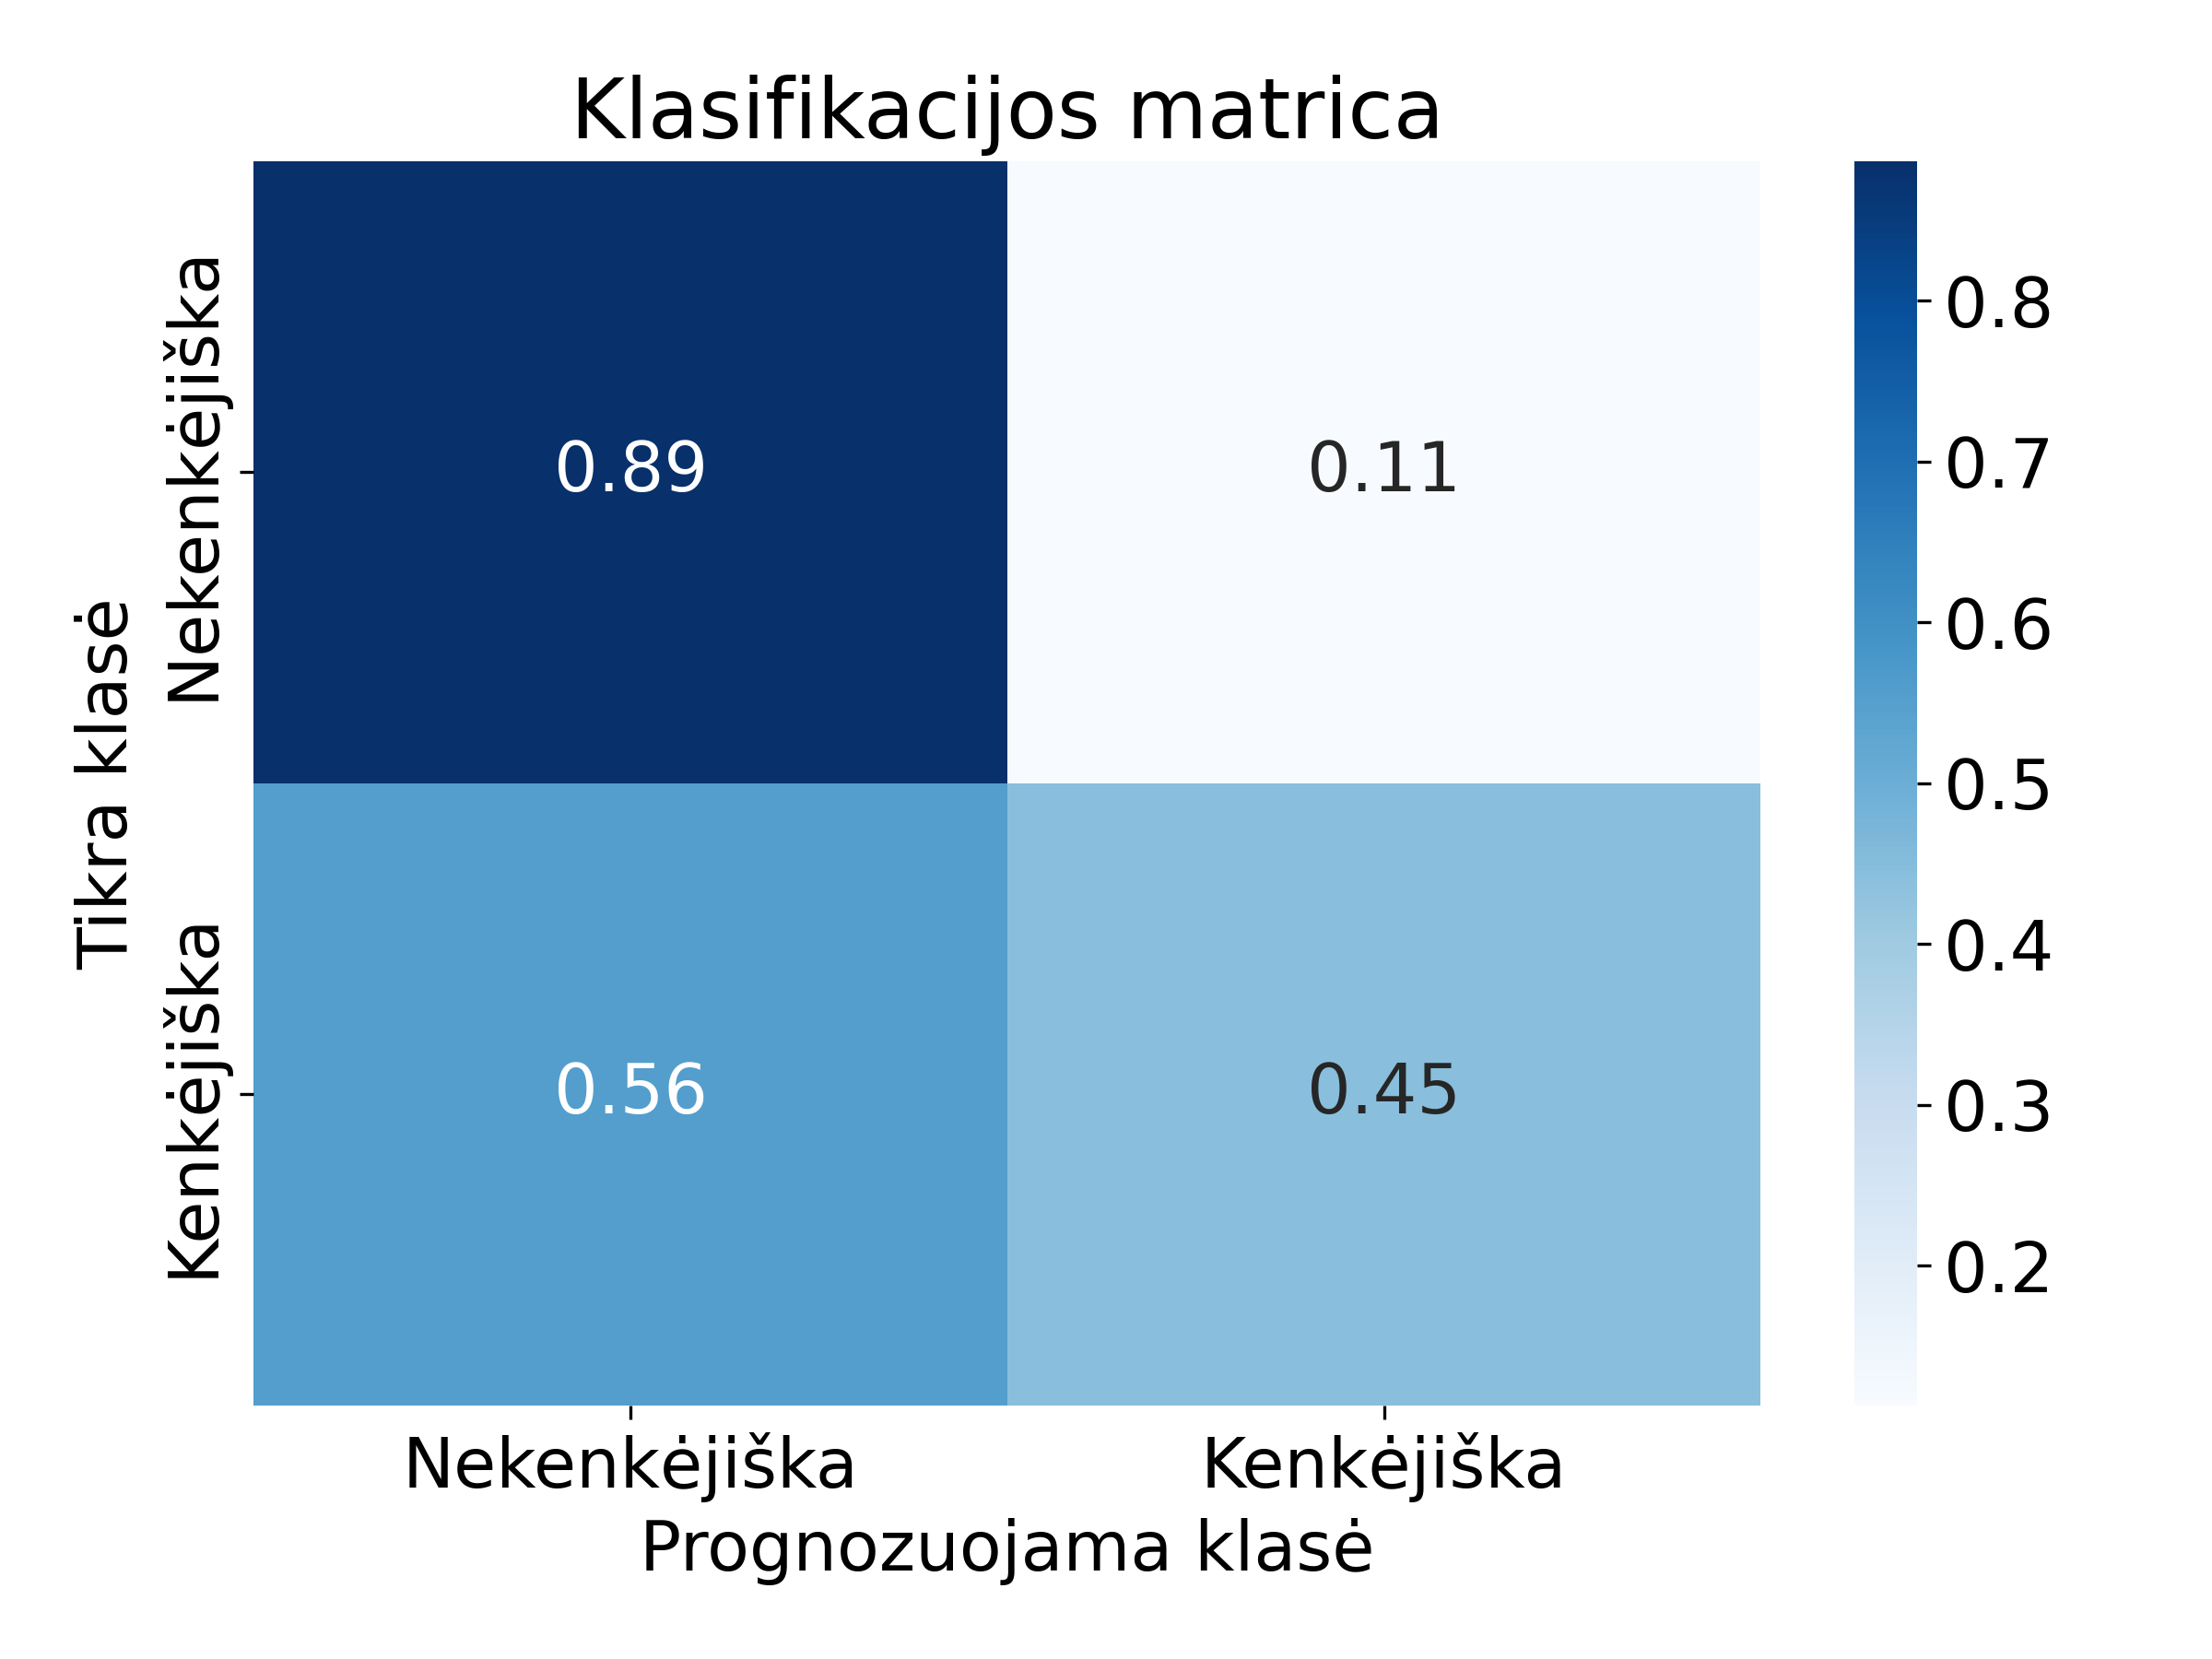
\includegraphics[width=0.45\textwidth]{images/normal_2x2.png}
    \caption{Klasifikavimo matrica}
    \label{fig:exp1:confusion}
\end{figure}

\begin{table}[h]
    \caption{Originalaus klasifikatoriaus metrikos}
    \centering
    \exptable[\accNormal]{tables/normal_2x2.csv}
    \label{tbl:exp1:metrics}
\end{table}
\clearpage
\subsubsection{\gls{mca} transformacijos klasifikatoriaus tikslumo nustatymas}\label{sec:exp:4}

\gls{mca} klasifikatorius yra vienas iš standartinių klasifikatorių (šiuo atveju atsitiktinio miško \angl{random forest}), naudojantis pakeistos bazės požymius kaip įvestį. Šioje vietoje naudojamas klasifikatorius gali būti bet koks, tačiau turi būti suderinamas su \gls{mca} komponenčių kiekio reikalavimais \skyrius{sec:method:mca_comp_selection}. 

Kaip ir originalus klasifikatorius, šis negeba išskirti obfuskuotų programų, tad \ref{fig:exp4:confusion} pav. pateikiamoje klasifikavimo lentelėje rodomas prognozuojamos klasės ir visų tai klasei priklausančių duomenų santykis.
Eksperimento rezultatai (klasifikavimo metrikos) pateikiami \ref{tbl:exp4:metrics}-oje lentelėje.
\begin{figure}[h]
    \centering
    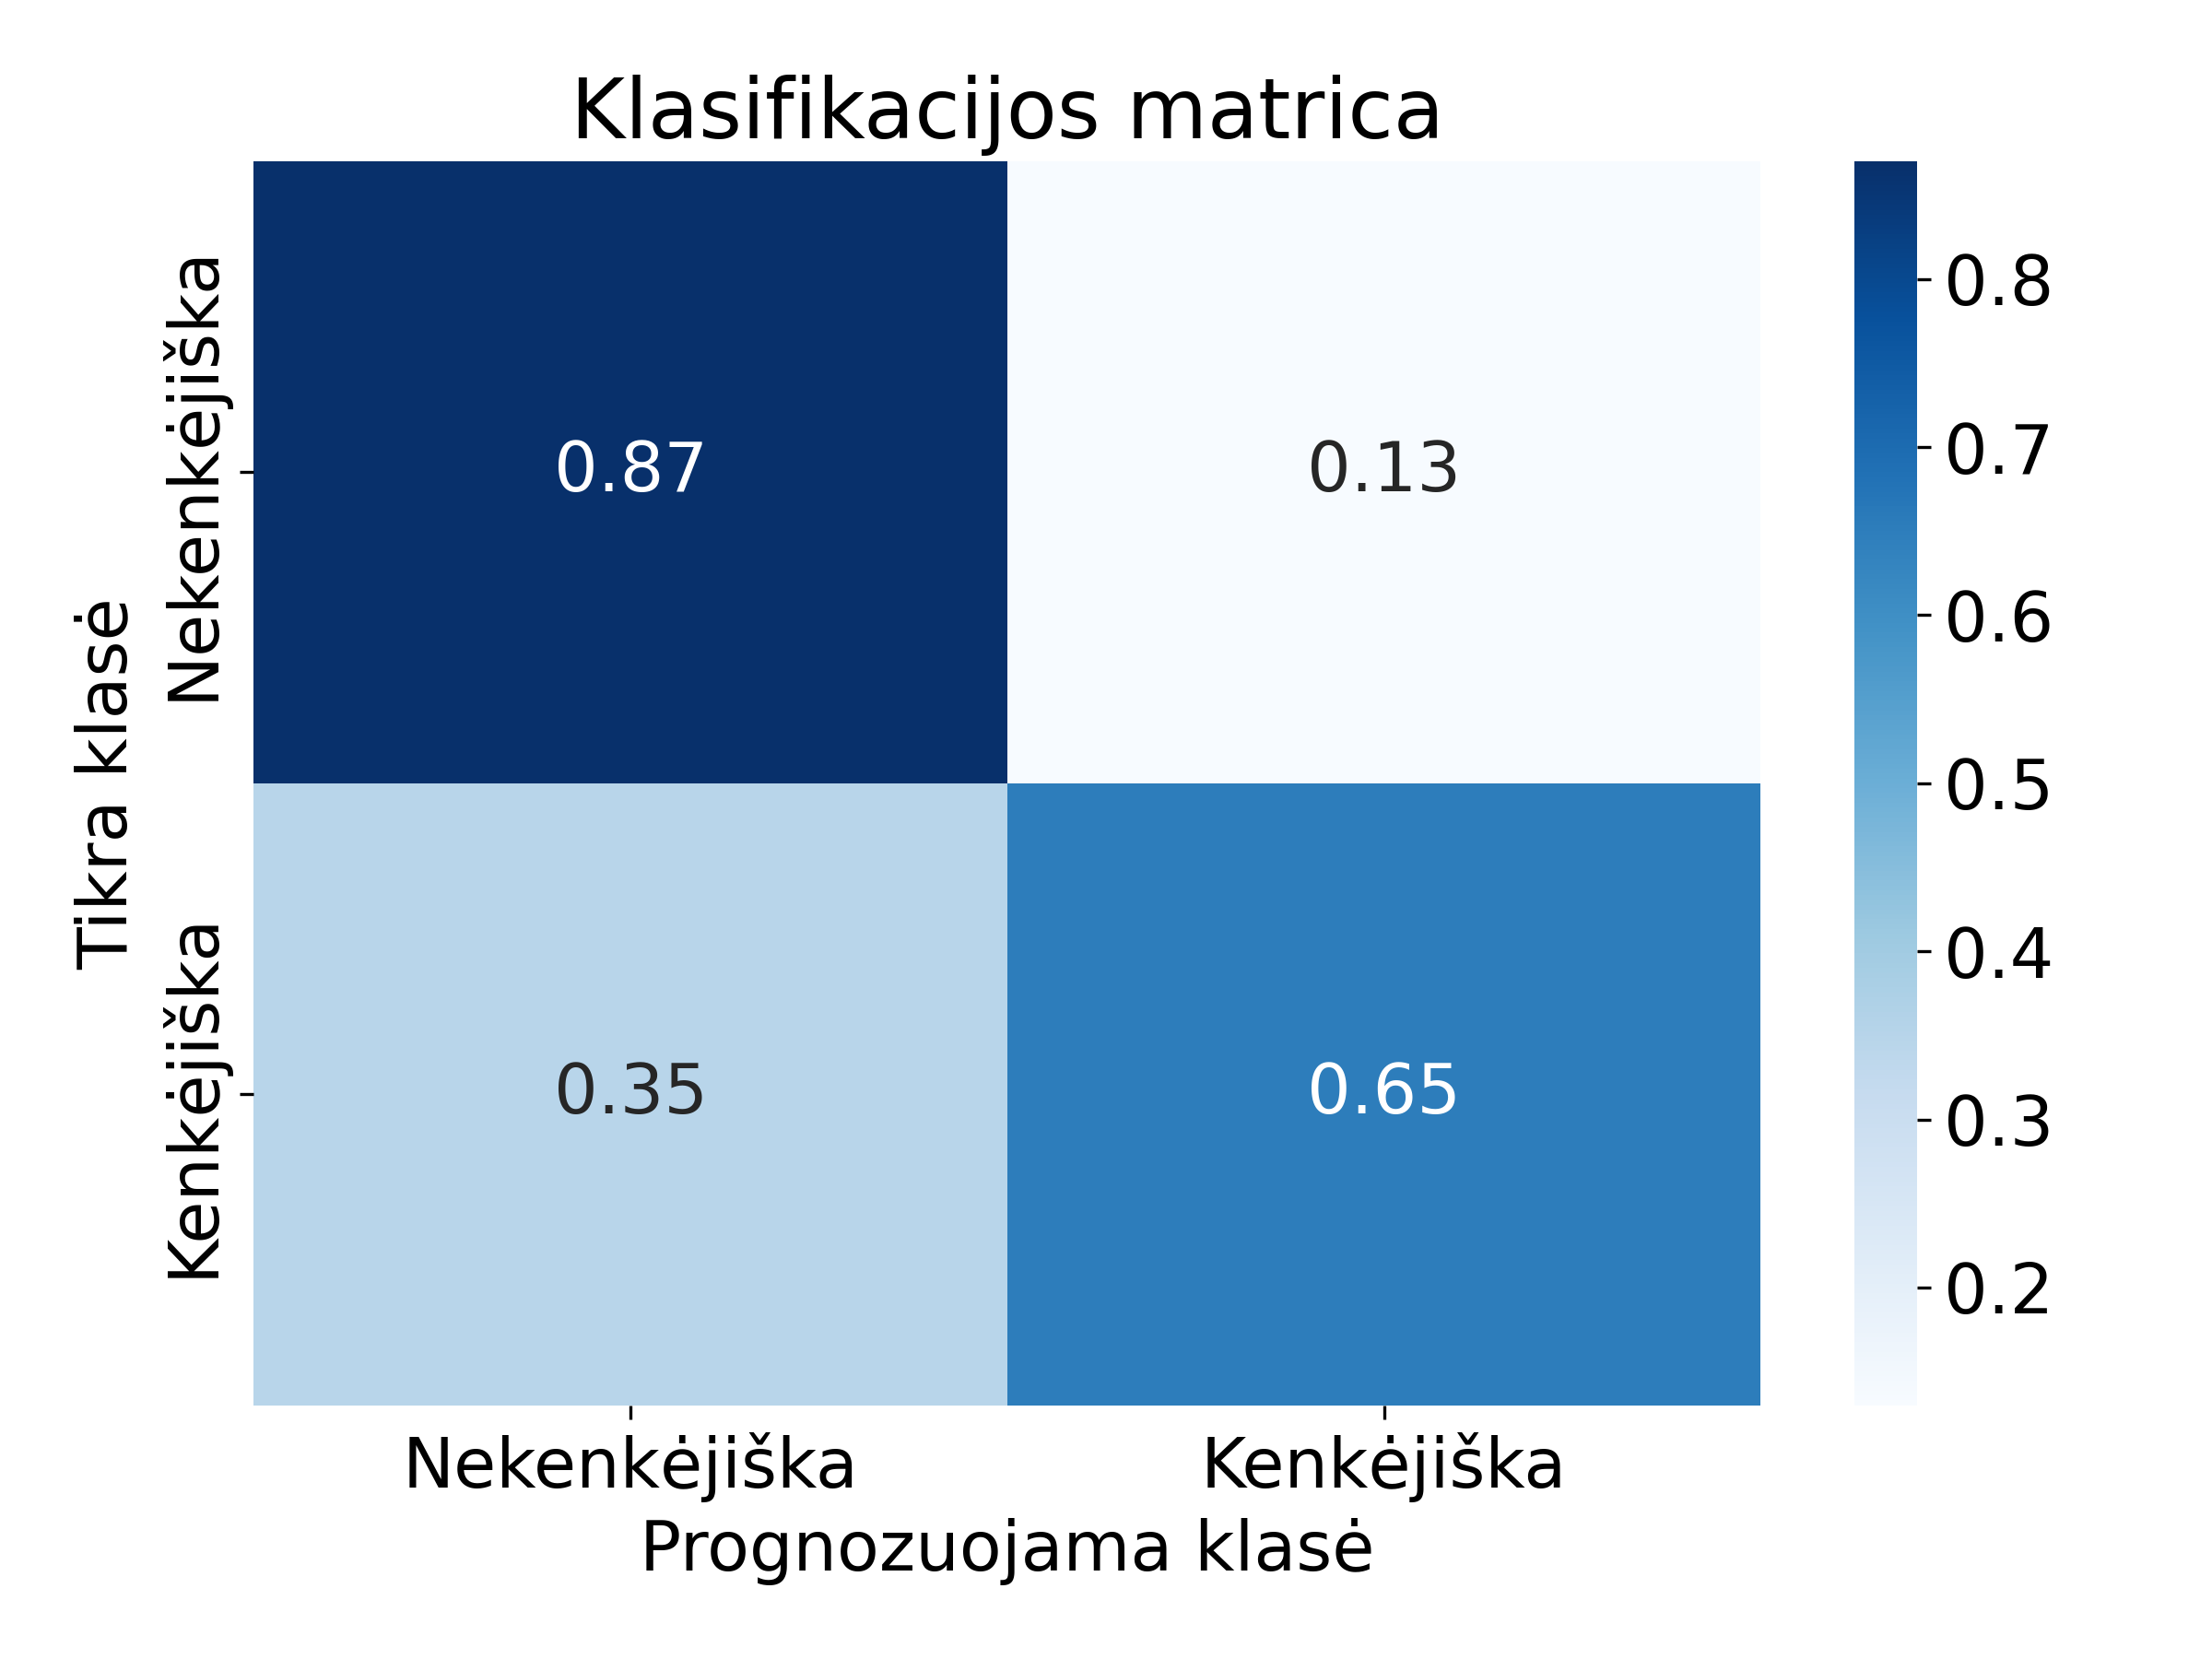
\includegraphics[width=0.5\textwidth]{images/mca_2x2.png}
    \caption{Klasifikavimo matrica}
    \label{fig:exp4:confusion}
\end{figure}

\begin{table}[h]
    \caption{\gls{mca} transformacijos klasifikatoriaus metrikos}
    \centering
    \exptable[\accMcaEquiv]{tables/mca_2x2.csv}
    \label{tbl:exp4:metrics}
\end{table}
\clearpage
\subsubsection{Modifikuoto \LIME pritaikymo \gls{ae} aptikimui tikslumo nustatymas}\label{sec:exp:2}

Šio eksperimento tikslas yra nustatyti modifikuoto \LIME pritaikymo \gls{ae} aptikimui \poskyris{sec:method:mods} tikslumą. \LIME branduolio plotis paliekamas pagal numatytus nustatymus ($\omega = 0,75 \cdot \sqrt{n}$, čia $n$ -- požymių skaičius, taigi, $\omega = 0,75 \cdot \sqrt{200} \approx 10,61$) \cite{ribeiroWhyShouldTrust2016}.

Kadangi šis metodas geba aptikti \gls{ae} -- obfuskuotas programas --
\ref{fig:exp2:confusion} pav. pateikiamos dvi klasifikacijos lentelės. Pirmoje (\ref{fig:exp2:confusion:a}) -- klasifikacijos rezultatai, kai obfuskuota programa laikoma kenkėjiška. Antroje (\ref{fig:exp2:confusion:b}) -- išskiriama \textit{obfuskuota} klasė. Kadangi išskyrus šią klasę duomenų rinkinys tampa subalansuotas, klasifikavimo lentelėje pateikiami sveiki skaičiai, atitinkantys modelio prognozuojamų duomenų tai klasei kiekį.

Eksperimento rezultatai (klasifikavimo metrikos) pateikiami \ref{tbl:exp2:metrics2}-oje ir \ref{tbl:exp2:metrics3}-oje lentelėse.
\begin{figure}[h]
    \begin{subfigure}{0.5\textwidth}
        \centering
        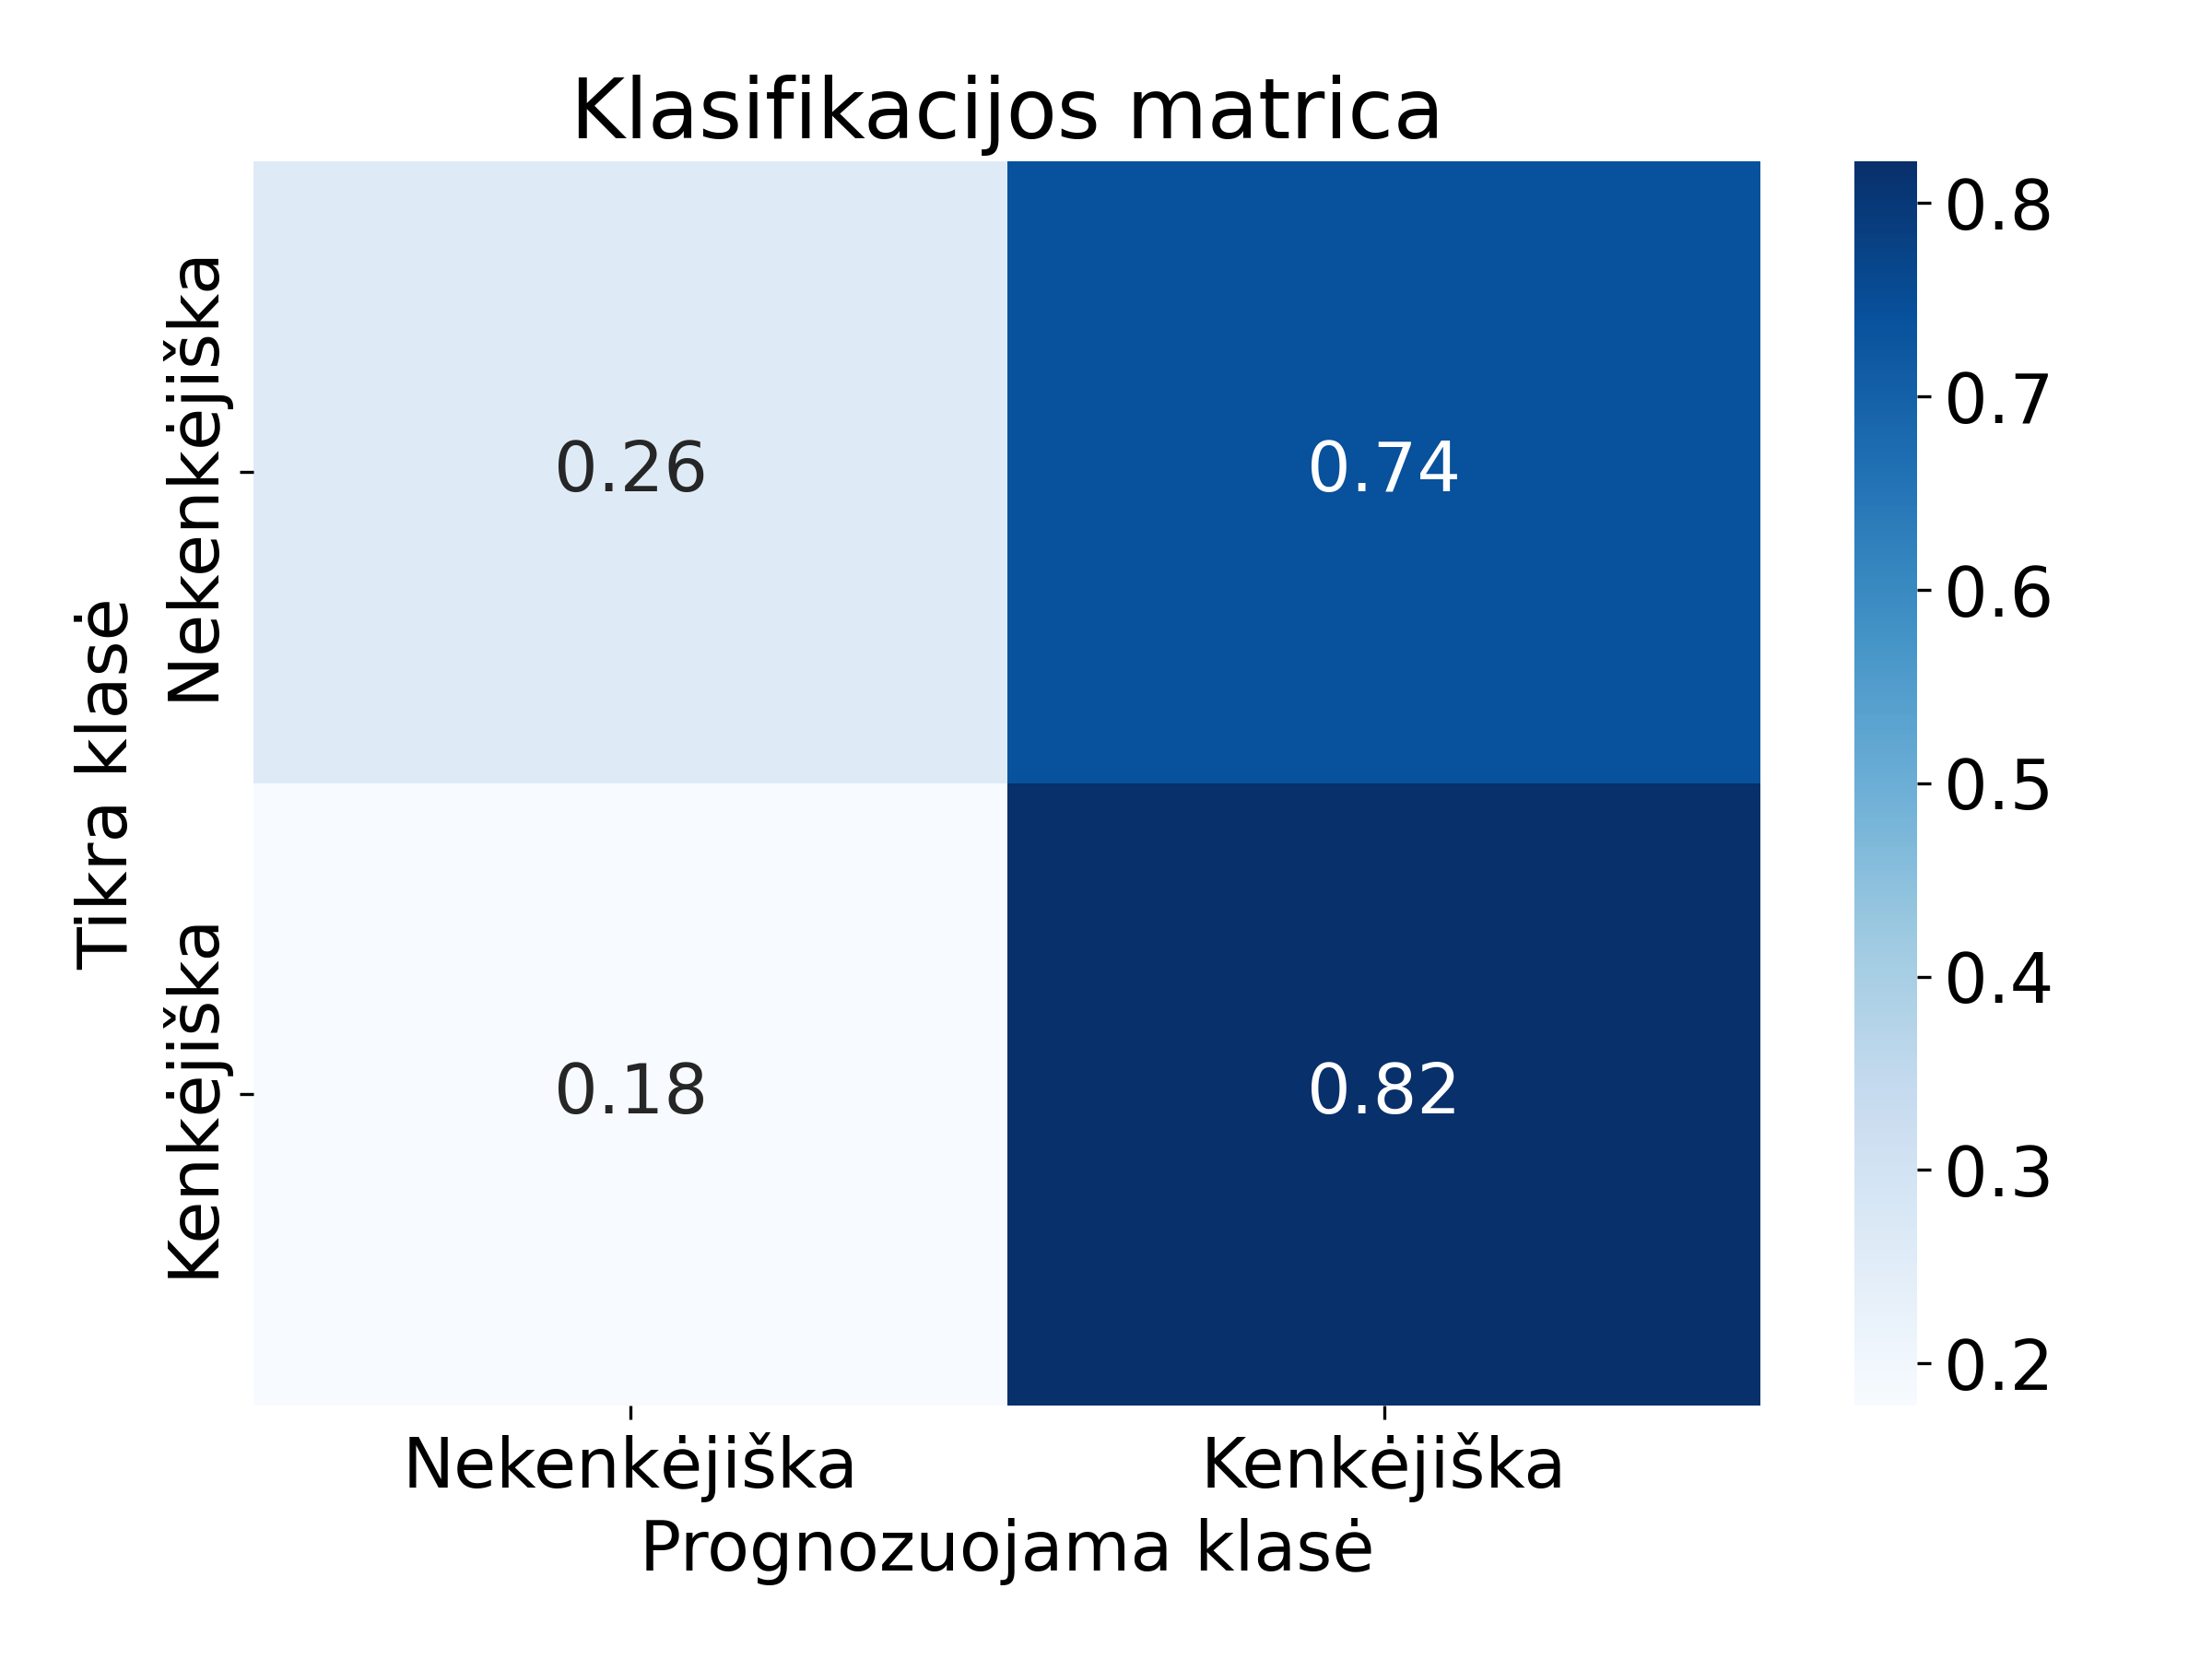
\includegraphics[width=\textwidth]{images/lime_2x2.png}
        \caption{Neišskiriant \textit{obfuskuotų} pavyzdžių klasės}
        \label{fig:exp2:confusion:a}
    \end{subfigure}
    \begin{subfigure}{0.5\textwidth}
        \centering
        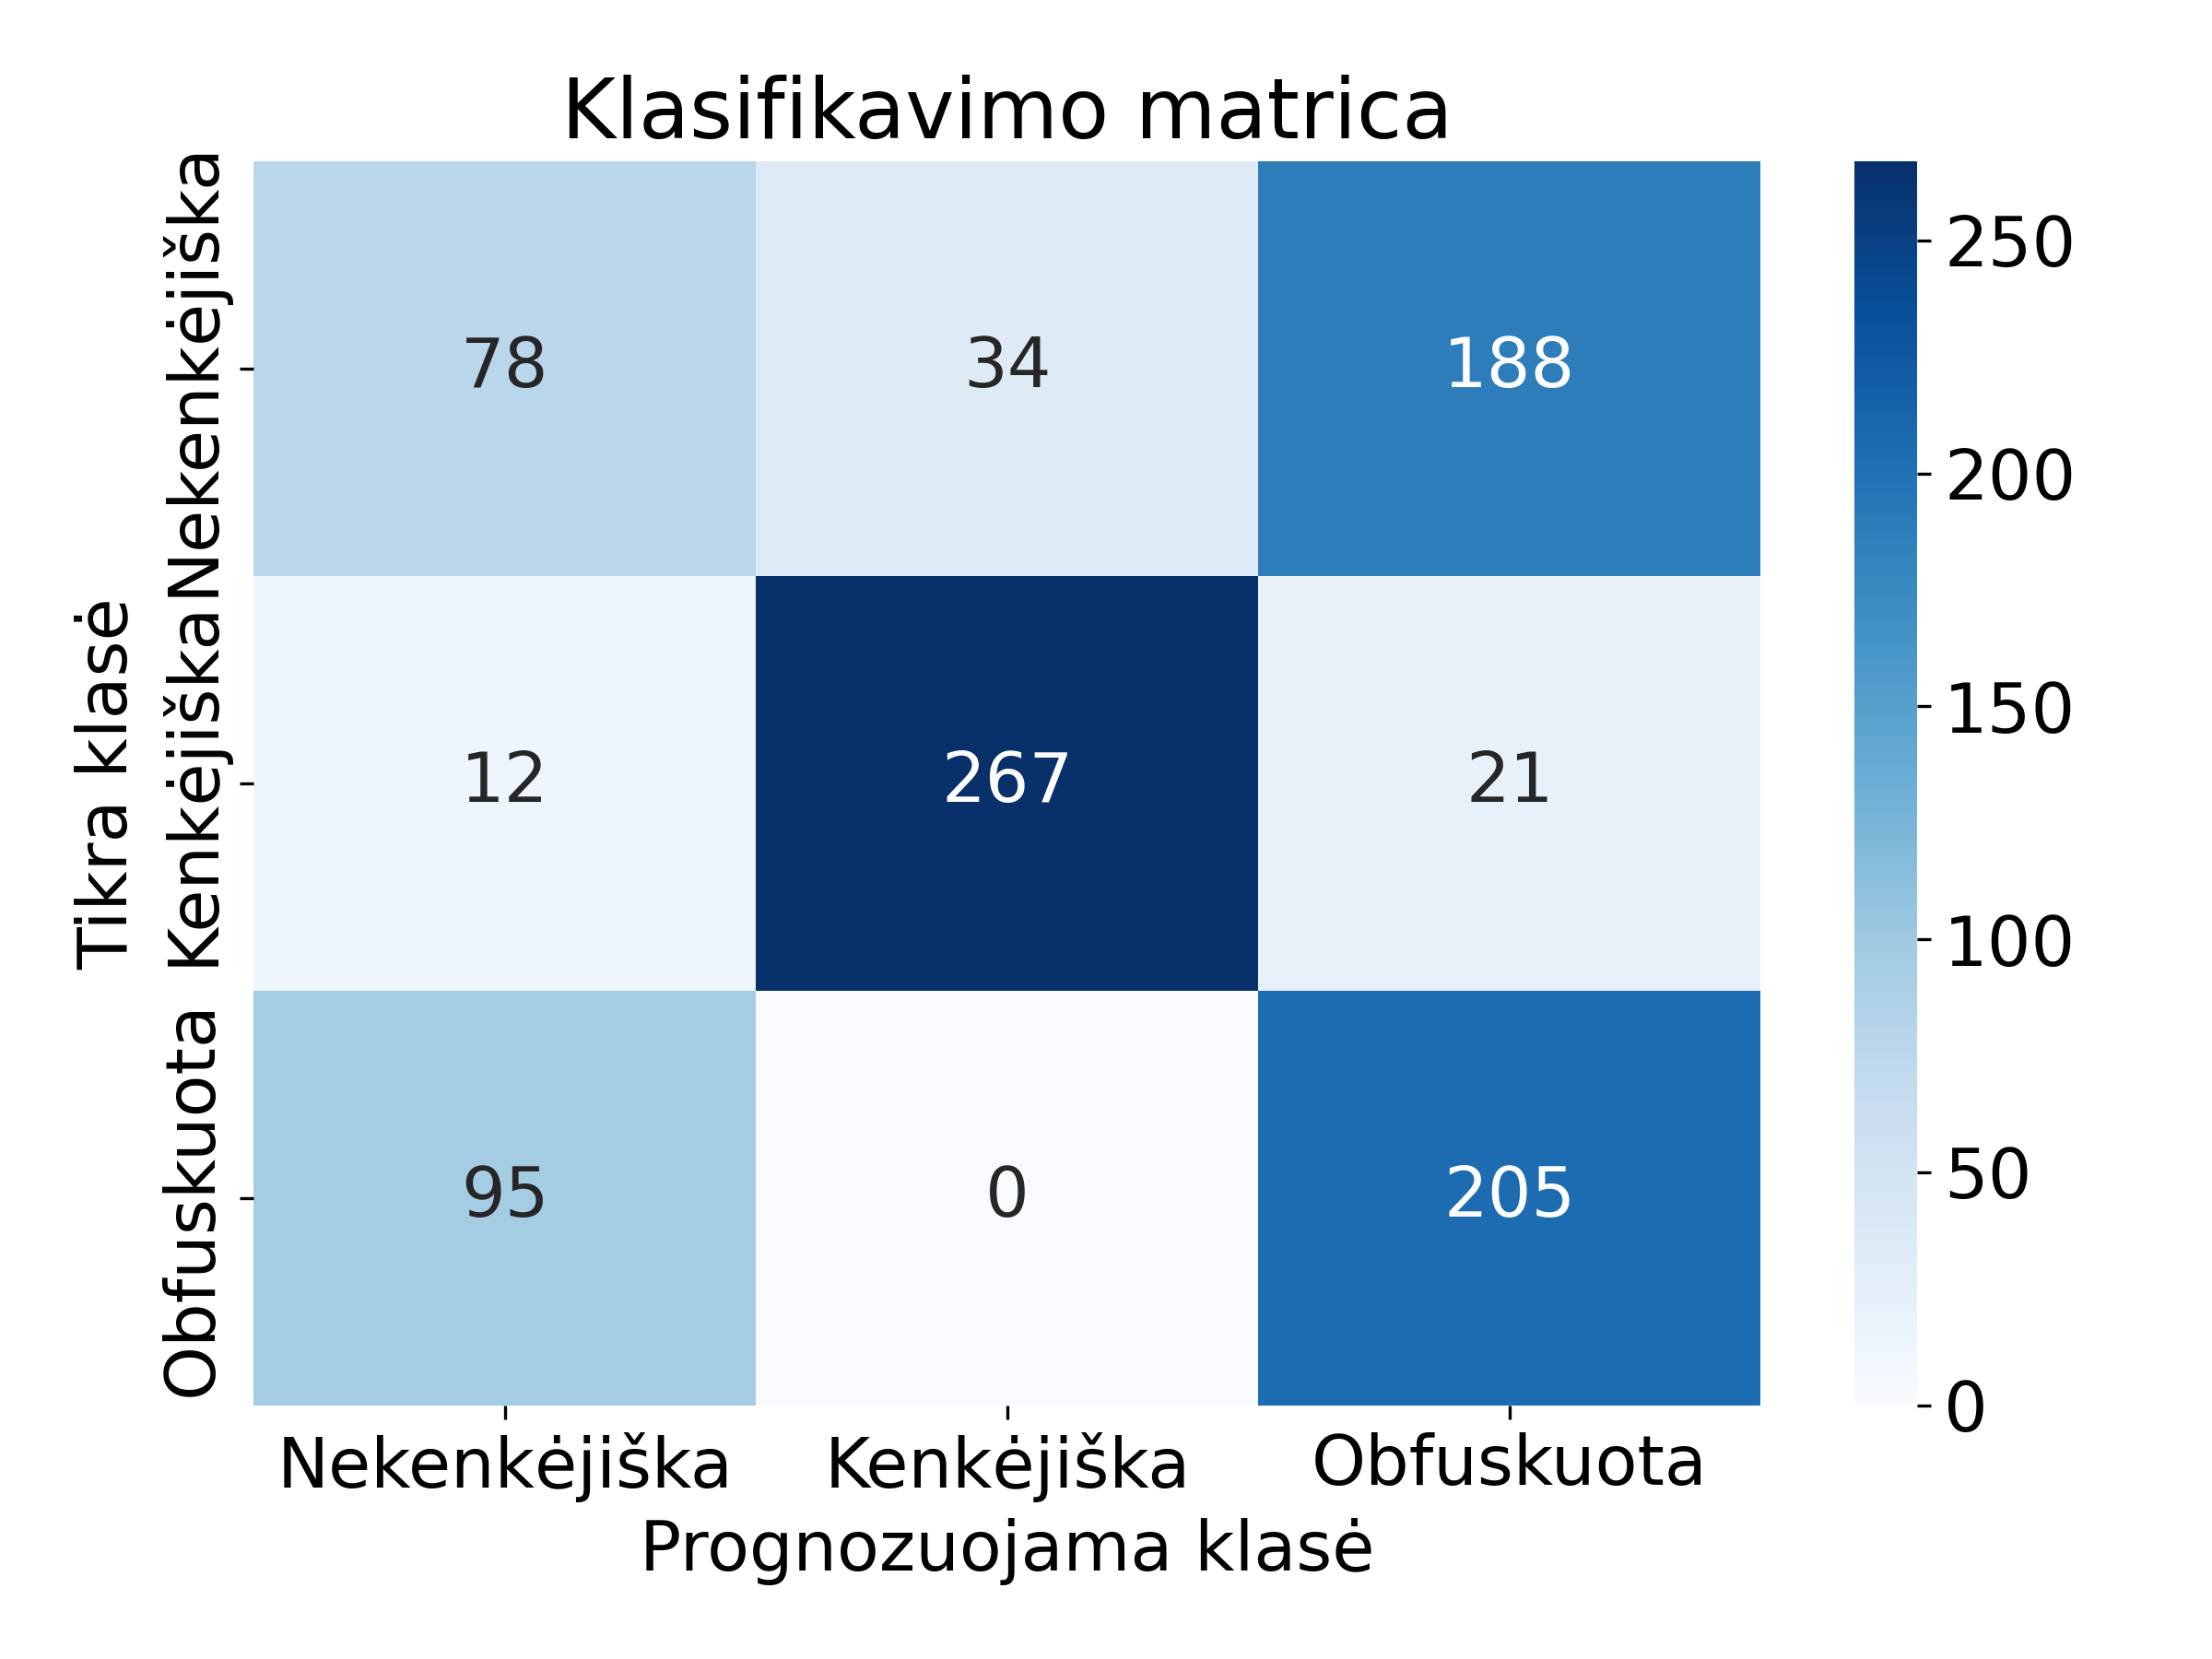
\includegraphics[width=\textwidth]{images/lime_3x3.png}
        \caption{Išskiriant \textit{obfuskuotų} pavyzdžių klasę}
        \label{fig:exp2:confusion:b}
    \end{subfigure}
    \caption{\LIME pritaikymo \gls{ae} aptikimui klasifikavimo lentelės}
    \label{fig:exp2:confusion}
\end{figure}

\begin{table}[h]
    \caption{\LIME pritaikymo \gls{ae} aptikimui klasifikatoriaus metrikos (neišskiriant \textit{obfuskuotos} klasės)}
    \centering
    \exptable[\accLimeCat]{tables/lime_2x2.csv}
    \label{tbl:exp2:metrics2}
\end{table}

\begin{table}[h]
    \caption{\LIME pritaikymo \gls{ae} aptikimui klasifikatoriaus metrikos (išskiriant \textit{obfuskuotą} klasę)}
    \centering
    \exptable[\accLimeCatObf]{tables/lime_3x3.csv}
    \label{tbl:exp2:metrics3}
\end{table}

% Use the paper method and show results that do not perform well
\clearpage
\subsubsection{\LIME ir \gls{mca} metodų sintezės tikslumo nustatymas}\label{sec:exp:3}

Šio eksperimento tikslas yra nustatyti autoriaus siūlomos modifikuoto \LIME ir \gls{mca} metodų sintezės \glsplko{adversarial} aptikimui tikslumą. Kaip ir praeitame eksperimente, \ref{fig:exp3:confusion}-ame pav. pateikiamos dvi klasifikavimo lentelės -- išskiriant ir neišskiriant \textit{obfuskuotą} klasę. 

Eksperimento rezultatai (klasifikavimo metrikos) pateikiami \ref{tbl:exp3:metrics2}-oje ir \ref{tbl:exp3:metrics3}-oje lentelėse.

\begin{figure}[h]
    \begin{subfigure}{0.5\textwidth}
        \centering
        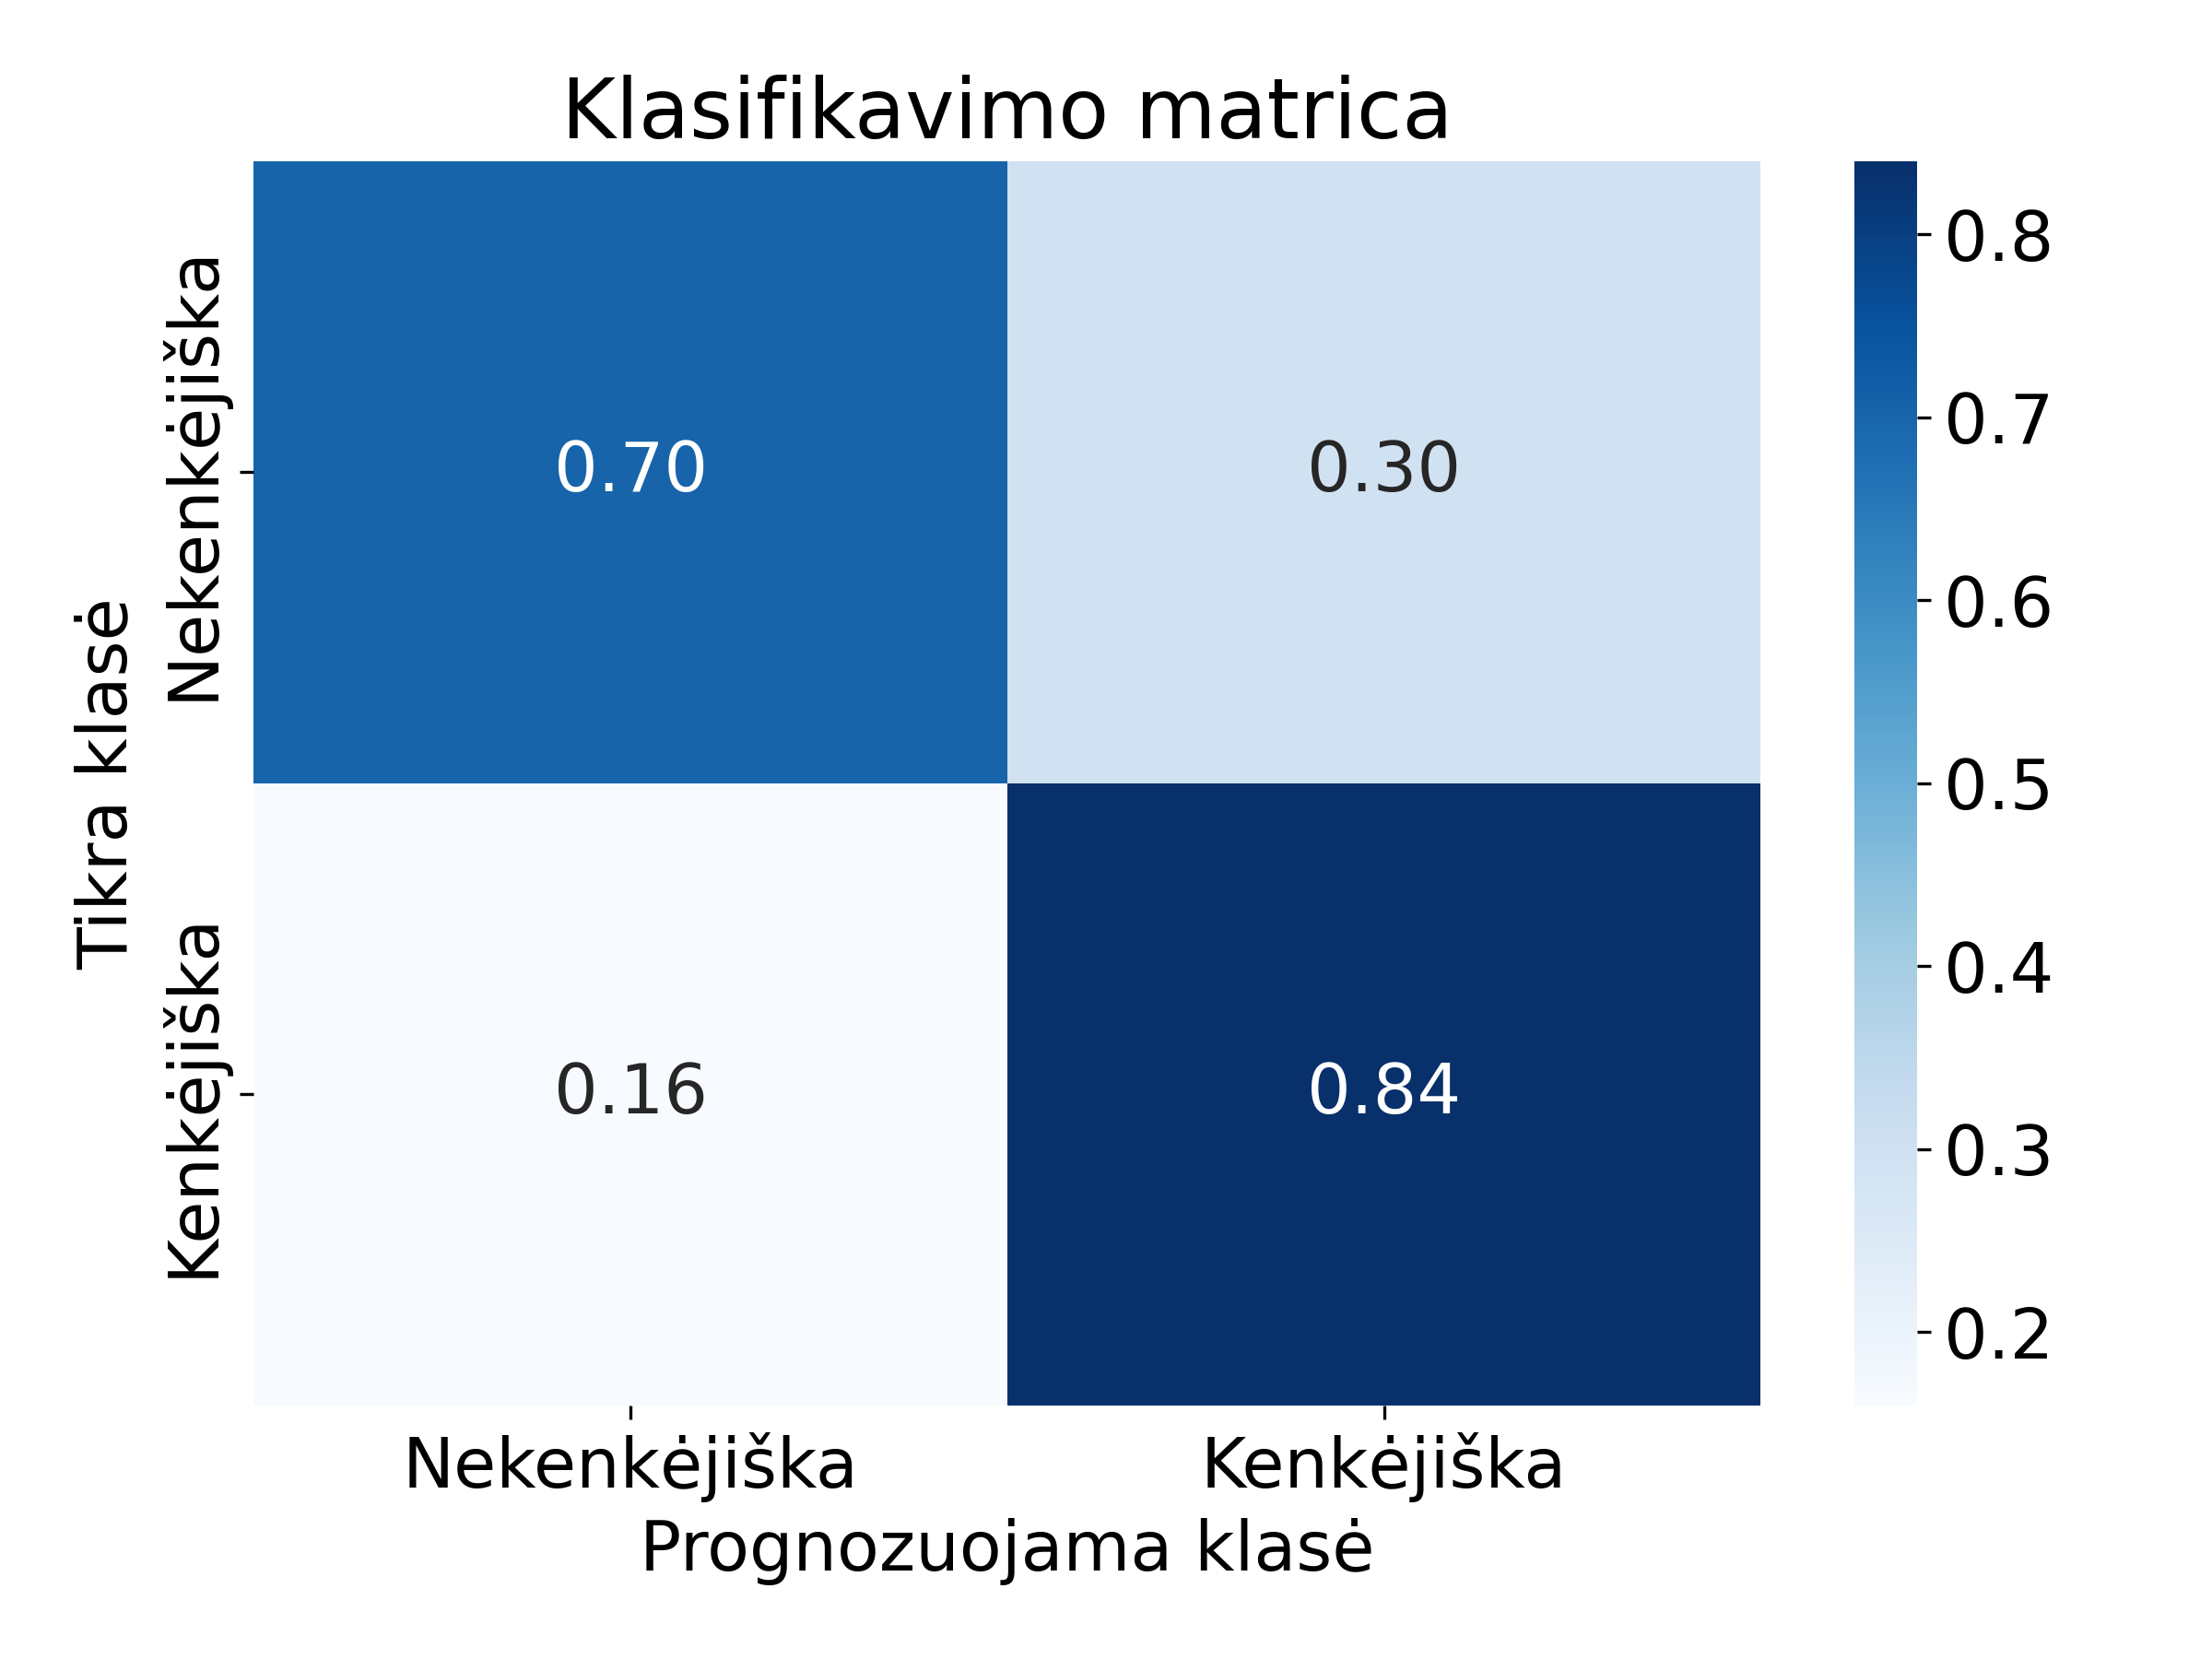
\includegraphics[width=\textwidth]{images/synthesis_2x2.png}
        \caption{Neišskiriant \textit{obfuskuotų} pavyzdžių klasės}
    \end{subfigure}
    \begin{subfigure}{0.5\textwidth}
        \centering
        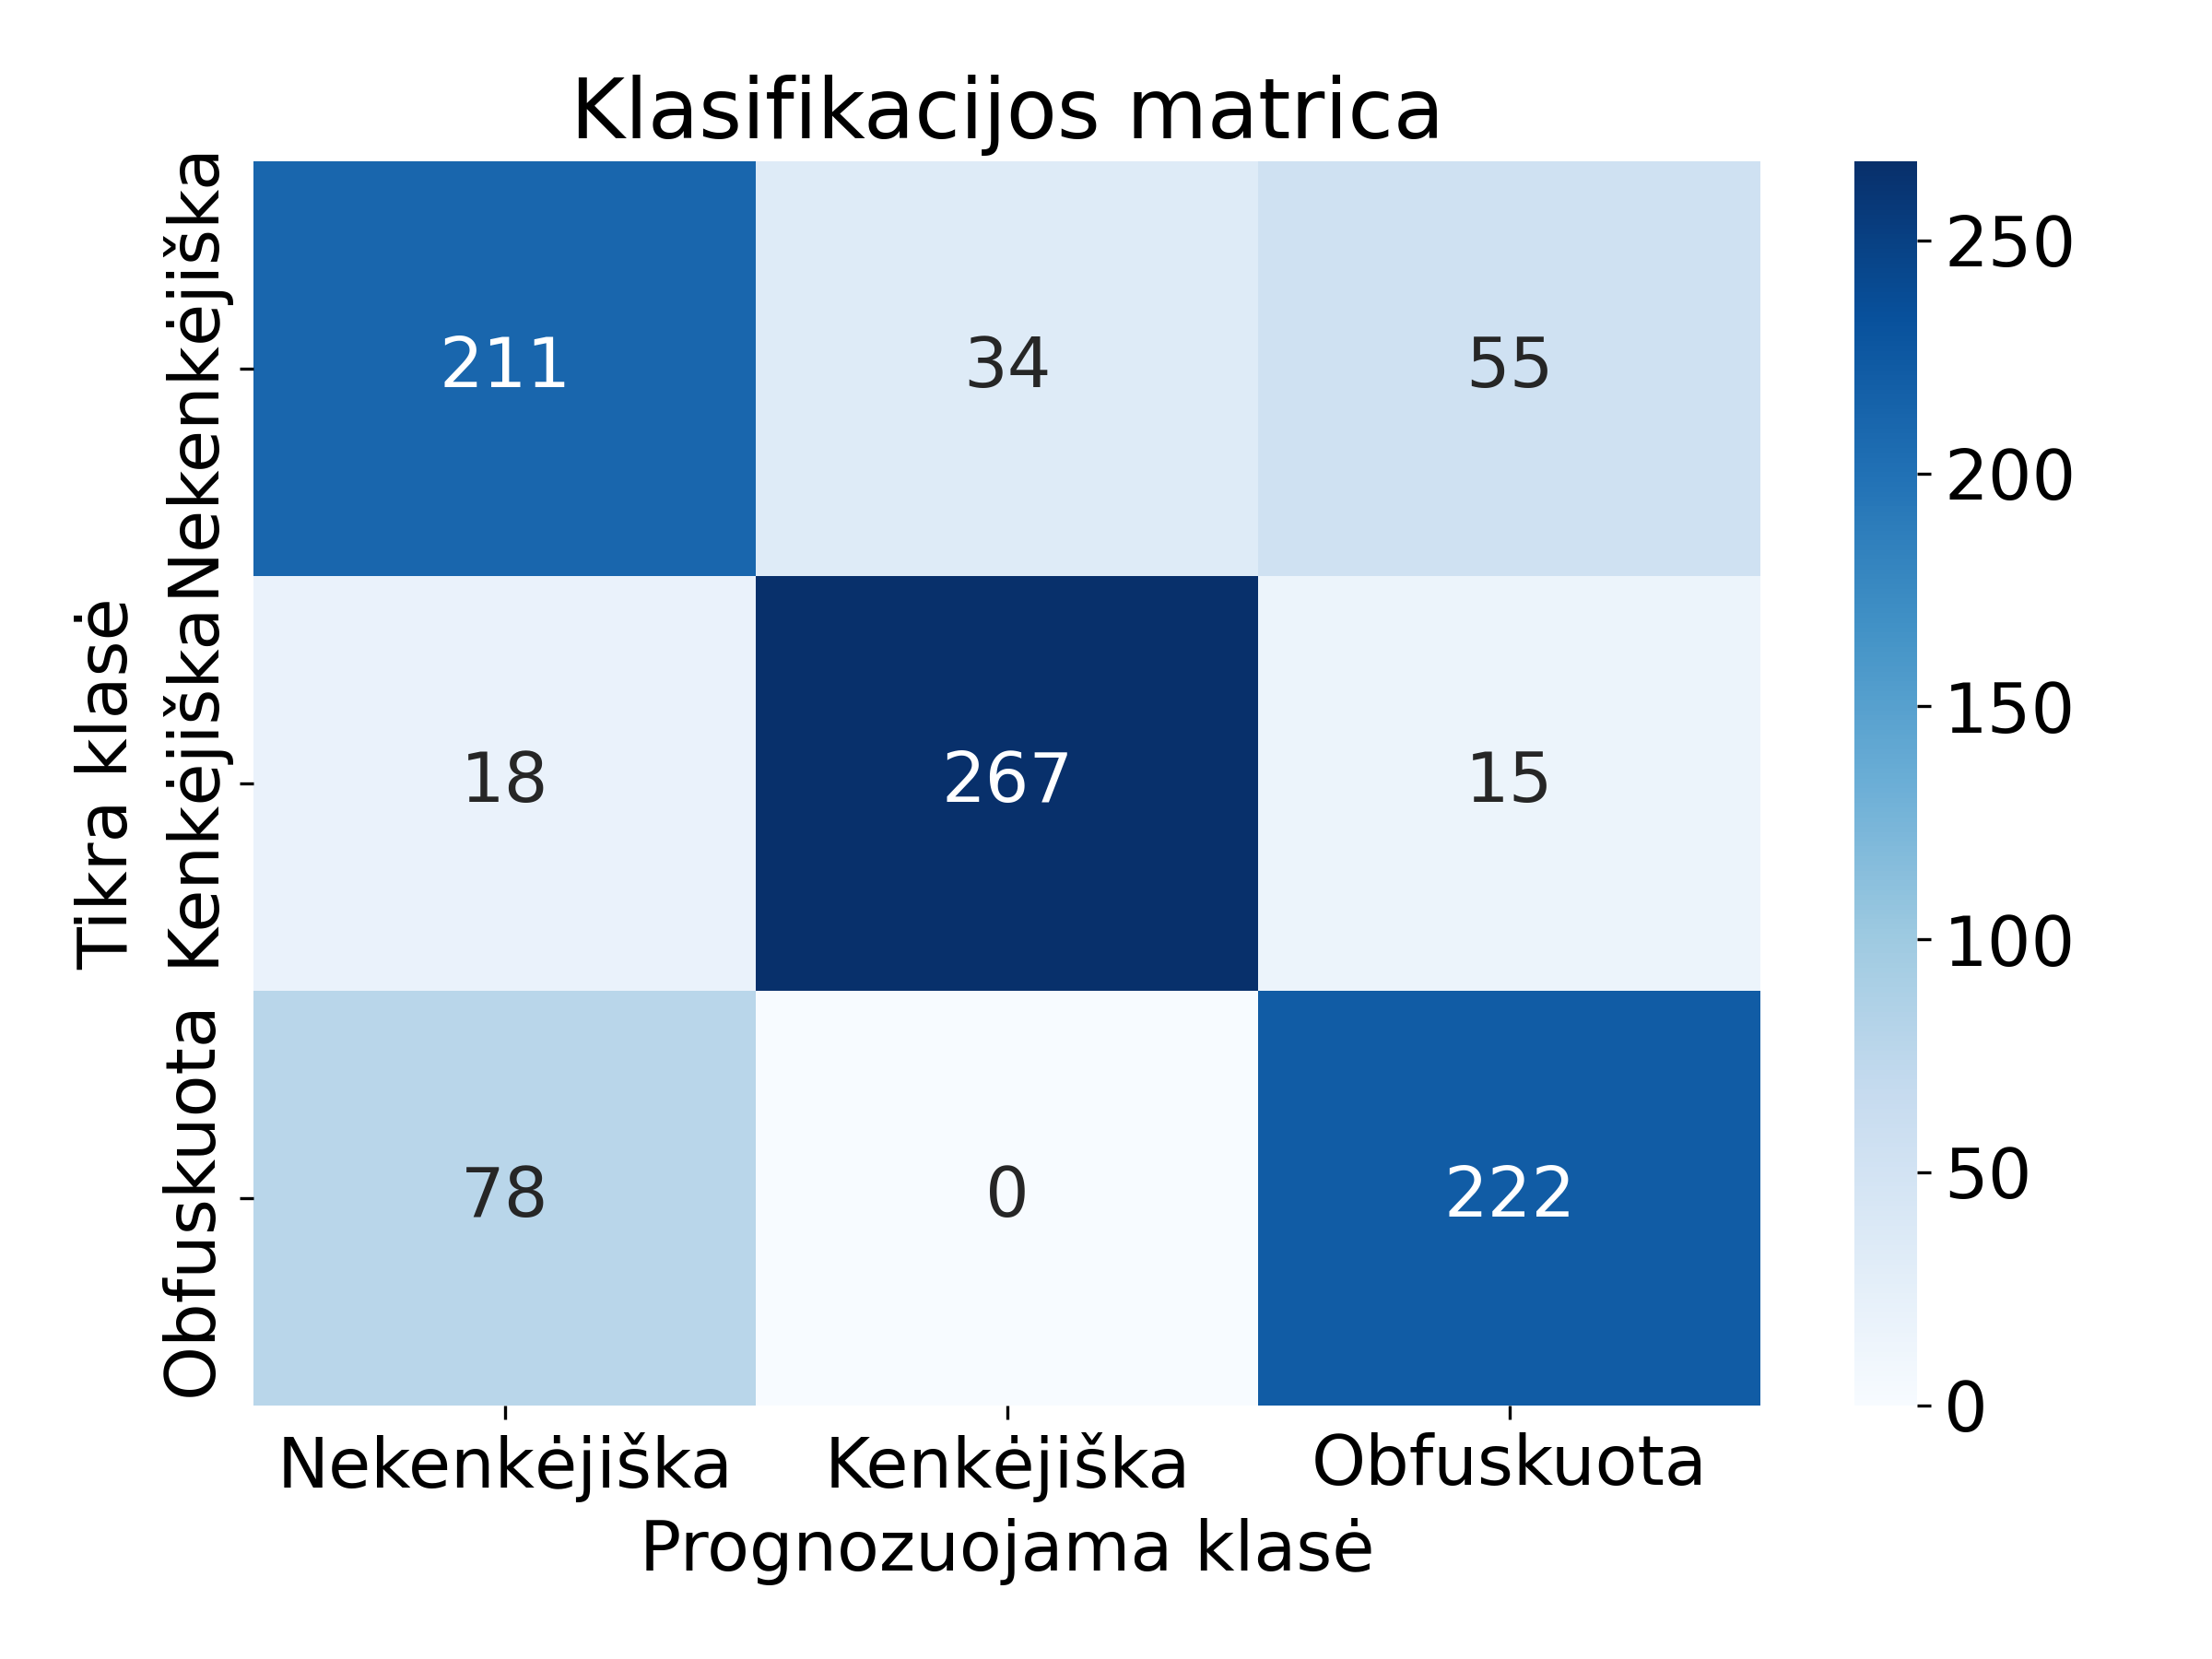
\includegraphics[width=\textwidth]{images/synthesis_3x3.png}
        \caption{Išskiriant \textit{obfuskuotų} pavyzdžių klasę}        
    \end{subfigure}
    \caption{\LIME ir \gls{mca} metodų sintezės klasifikavimo lentelės}
    \label{fig:exp3:confusion}
\end{figure}

\begin{table}[h]
    \caption{\LIME ir \gls{mca} metodų sintezės klasifikatoriaus metrikos (neišskiriant \textit{obfuskuotos} klasės)}
    \centering
    \exptable[\accLime]{tables/synthesis_2x2.csv}
    \label{tbl:exp3:metrics2}
\end{table}

\begin{table}[h]
    \caption{\LIME ir \gls{mca} metodų sintezės klasifikatoriaus metrikos (išskiriant \textit{obfuskuotą} klasę)}
    \centering
    \exptable[\accLimeObf]{tables/synthesis_3x3.csv}
    \label{tbl:exp3:metrics3}
\end{table}

\section{Rezultatai ir išvados}

\subsection*{Rezultatai}

Atlikus tyrimą, gauti šie rezultatai:

\begin{enumerate}
    \item Apžvelgti ir pritaikyti mokslinėje literatūroje minimi kodo obfuskacijos bei \glsplko{adversarial} -- \gls{ae} generavimo -- metodai, jų aptikimo strategijos \skyrius{sec:literature}.
    \item Pasiūlytas naujas \gls{ae} aptikimo metodas, pritaikomas bet kokiam kenkėjiškų programų detektoriui bei gebantis apdoroti dvejetainius požymius, apjungiantis \LIME pritaikymo \gls{ae} aptikimui ir \gls{mca} transformacijos idėjas \skyrius{sec:method}.
    \item Atliktas \gls{ae} aptikimo metodų lyginamosios analizės tyrimas \skyrius{sec:experiments} ir nustatytas pasiūlyto \gls{ae} aptikimo metodo \skyrius{sec:method} efektyvumas (matuojant modelio tikslumą ir atsižvelgiant į kitas klasifikacijos metrikas), lyginant pasiūlytą metodą su jo sudedamosiomis dalimis \Zr{tbl:exp:summary}.
\end{enumerate}

\begin{table}[h]
    \centering
    \caption{Eksperimentų rezultatų (tikslumo metrikų) suvestinė}
    \begin{tabular}{l|c|c|r}
        \bfseries Eksperimentas &\bfseries Tikslumas (K/N)\footnotemark &\bfseries Tikslumas (K/N/O)\footnotemark & $\Delta a\footnotemark,\;\%$ \\ \hline
        \ref{sec:exp:1} Bazinis & \num{\accNormal} & - & $\num{\mathOp{(\accNoAttackNormal - \accNormal)*100}}$ \\
        \ref{sec:exp:4} \gls{mca} & \num{\accMcaEquiv} & - & $\num{\mathOp{(\accNoAttackNormal - \accMcaEquiv)*100}}$ \\
        \ref{sec:exp:2} \LIME & \num{\accLimeCat} & \num{\accLimeCatObf} & $\num{\mathOp{(\accNoAttackNormal - \accLimeCat)*100}}$ \\
        \ref{sec:exp:3} \LIME + \gls{mca} & \num{\accLime} & \num{\accLimeObf} & $\num{\mathOp{(\accNoAttackNormal - \accLime)*100}}$ \\
    \end{tabular}
    \label{tbl:exp:summary}
\end{table}

\subsection*{Išvados}

\begin{enumerate}
    \item Autoriaus siūlomas \gls{ae} aptikimo metodas lyginamosios analizės tyrime pasiekė geriausią rezultatą (didžiausią tikslumą: \num{\mathOp{\accLime*100}} \% (\textbf{K/N}) ir \num{\mathOp{\accLimeObf*100}} \% (\textbf{K/N/O})). Taip pat buvo pranašesnis už likusius modelius visomis kitomis lyginamomis metrikomis (preciziškumu, atkūrimu ir F1).
    \item Autoriaus siūlomo metodo $\Delta a$ yra mažiausia, taigi, tiek \glsplko{adversarial} aptikimo logika, tiek pačios \glspl{adversarial} turi palyginti mažą įtaką šio klasifikatoriaus tikslumui.
    \item Autoriaus siūlomas metodas aptinka 3 iš 4 \glsplko{adversarial} su $\num{76}\;\%$ preciziškumu. Lyginant su \LIME metodo pritaikymu \gls{ae} aptikimui (vieninteliu kitu metodu iš nagrinėtų, gebančiu aptikti \textit{obfuskuotą} klasę), atakų aptikimo santykis yra panašus, tačiau \LIME metodo pritaikymo preciziškumas -- tik $\num{49,5}\;\%$.
\end{enumerate}



\addtocounter{footnote}{-2}
\footnotetext{Kenkėjiška / Nekenkėjiška}
\stepcounter{footnote}
\footnotetext{Kenkėjiška / Nekenkėjiška / Obfuskuota}
\stepcounter{footnote}
\footnotetext{Skirtumas tarp originalaus klasifikatoriaus tikslumo aplinkoje be \glsplko{adversarial} \Zr{tbl:safe:original:metrics} ir \textbf{tikslumo (K/N)} aplinkoje su \glsplkuo{adversarial}}

\setlength{\bibitemsep}{0pt plus 0.3ex}
\printbibliography[heading=bibintoc,title = {Literatūra ir šaltiniai}]


\end{document}
